\documentclass[handout]{beamer}

\mode<presentation>
{
    \usetheme{rwth}
    \setbeamercovered{transparent = 20}
}

\usepackage{graphicx}
\usepackage[utf8]{inputenc}
\usepackage{enumitem}
\usepackage{hyperref}
\usepackage{listings}

\usepackage[section]{algorithm}
\usepackage{packages/algo}

\usepackage{array}
\setlength\extrarowheight{2pt}

\usepackage[FIGTOPCAP]{subfigure}
\usepackage{tikz}
\usetikzlibrary{calc}
\usetikzlibrary{matrix}
\usepackage{pgfplots}
\usepackage{pgfplotstable}
\usepackage{multirow}
% using equal sign in column labels
\newcommand{\pgfequalsign}{=}
\newcommand\refbsdnyu[1]{% positions two related legendimages in one cell
  \raisebox{1.5pt}{\ref{plot:#1bsd}}\llap{\raisebox{-1pt}{\ref{plot:#1nyu}}}%
}
\pgfplotscreateplotcyclelist{comparison bsd 1}{%
	blue,mark=star,solid\\% oriSEEDS
	red,mark=star,solid\\% reSEEDS
} 
\pgfplotscreateplotcyclelist{comparison bsd 2}{%
	teal,mark=star,solid\\% SLIC
	blue,mark=star,solid\\% oriSEEDS
	red,mark=star,solid\\% reSEEDS
}
\pgfplotscreateplotcyclelist{comparison bsd 3}{%
	orange,mark=star,solid\\% FH
	teal,mark=star,solid\\% SLIC
	blue,mark=star,solid\\% oriSEEDS
	red,mark=star,solid\\% reSEEDS
}
\pgfplotscreateplotcyclelist{comparison nyu 1}{%
	blue,mark=star,solid\\% oriSEEDS
	red,mark=star,solid\\% reSEEDS
	red,mark=star,dashed\\% SEEDS3D
}
\pgfplotscreateplotcyclelist{comparison nyu 2}{%
	orange,mark=star,solid\\% FH
	teal,mark=star,solid\\% SLIC
	blue,mark=star,solid\\% oriSEEDS
	red,mark=star,solid\\% reSEEDS
	red,mark=star,dashed\\% SEEDS3D
}
\pgfplotscreateplotcyclelist{comparison nyu 3}{%
	orange,mark=star,solid\\% FH
	teal,mark=star,solid\\% SLIC
	blue,mark=star,solid\\% oriSEEDS
	red,mark=star,solid\\% reSEEDS
	red,mark=star,dashed\\% SEEDS3D
	brown,mark=star,dashed\\% VCCS
}
\pgfplotscreateplotcyclelist{runtime bsd}{%
	orange,mark=star,solid\\% FH
	teal,mark=star,solid\\% SLIC
	blue,mark=star,solid\\% oriSEEDS
	red,mark=star,solid\\% reSEEDS
}
\pgfplotscreateplotcyclelist{runtime nyu}{%
	orange,mark=star,solid\\% FH
	teal,mark=star,solid\\% SLIC
	blue,mark=star,solid\\% oriSEEDS
	red,mark=star,solid\\% reSEEDS
	red,mark=star,dashed\\% SEEDS3D
	brown,mark=star,dashed\\% VCCS
}
\pgfplotscreateplotcyclelist{low runtime bsd 1}{%
	teal,mark=star,solid\\% SLIC
	blue,mark=star,solid\\% oriSEEDS
	red,mark=star,solid\\% reSEEDSmp*
}
\pgfplotscreateplotcyclelist{low runtime bsd 2}{%
	teal,mark=star,solid\\% SLIC
	blue,mark=star,solid\\% oriSEEDS
	red,mark=star,solid\\% reSEEDSmp*
	teal,mark=diamond,solid\\% SLIC
	blue,mark=diamond,solid\\% oriSEEDS
	red,mark=diamond,solid\\% reSEEDSmp*
}
\pgfplotscreateplotcyclelist{low runtime nyu 1}{%
	teal,mark=star,solid\\% SLIC
	blue,mark=star,solid\\% oriSEEDS
	red,mark=star,solid\\% reSEEDSmp*
}
\pgfplotscreateplotcyclelist{low runtime nyu 2}{%
	teal,mark=star,solid\\% SLIC
	blue,mark=star,solid\\% oriSEEDS
	red,mark=star,solid\\% reSEEDSmp*
	teal,mark=diamond,solid\\% SLIC
	blue,mark=diamond,solid\\% oriSEEDS
	red,mark=diamond,solid\\% reSEEDSmp*
}
\pgfplotscreateplotcyclelist{comparison bsd full}{%
	orange,mark=star,solid\\% FH
	green!40!black,mark=star,solid\\% TP
	teal,mark=star,solid\\% SLIC
	cyan,mark=star,solid\\% ERS
	blue,mark=star,solid\\% oriSEEDS
	red,mark=star,solid\\% reSEEDS
}
\pgfplotscreateplotcyclelist{comparison nyu full}{%
	orange,mark=star,solid\\% FH
	green!40!black,mark=star,solid\\% TP
	teal,mark=star,solid\\% SLIC
	cyan,mark=star,solid\\% ERS
	blue,mark=star,solid\\% oriSEEDS
	red,mark=star,solid\\% reSEEDS
	red,mark=star,dashed\\% SEEDS3D
	violet,mark=star,dashed\\% DASP
	brown,mark=star,dashed\\% VCCS
}

\pgfplotsset{every axis/.append style={tick label style={/pgf/number format/fixed},font=\small,ylabel near ticks,xlabel near ticks,grid=major,mark options={scale=1.5}}}

\title{Superpixel Segmentation using Depth Information}
\author{David Stutz}
\date{October 7th, 2014}

\RWTHtoc{Table of Contents}
\begin{document}

	\RWTHtitle

	\begin{frame}{Table of Contents}
		\tableofcontents
	\end{frame}

	\section{Introduction}
	\begin{frame}{Introduction -- Superpixels}
		The term superpixel was coined by Ren and Malik \cite{RenMalik:2003} to describe a group of pixels perceptually belonging together:
		\vskip 0.25cm
		\begin{itemize}[label=--]
			\item Color similarity
			\item Spatial proximity
		\end{itemize}
		\vskip 0.5cm
		\pause
		
		Why are we interested in superpixels?
		\vskip 0.25cm
		\begin{itemize}[label=--]
			\item Pixels are only a result of discretization.
			\item The number of primitives is highly reduced.
		\end{itemize}
		\vskip 0.5cm
	\end{frame}
	
%	\begin{frame}{Introduction -- Superpixels}
%		\begin{figure}
%   			\centering
%   			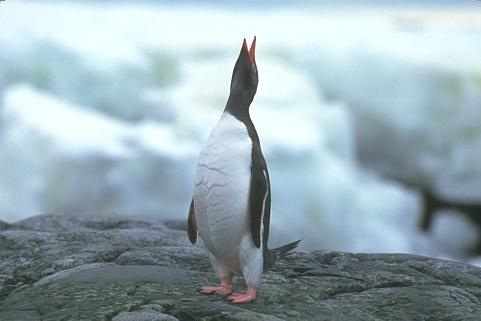
\includegraphics[scale=0.5]{images/bsd-2}
%   			\caption{Example image from the Berkeley Segmentation Dataset \cite{ArbelaezMaireFowlkesMalik:2011}.}
%   		\end{figure}
%	\end{frame}
%	
%	\begin{frame}{Introduction -- Superpixels}
%		\begin{figure}
%   			\centering
%   			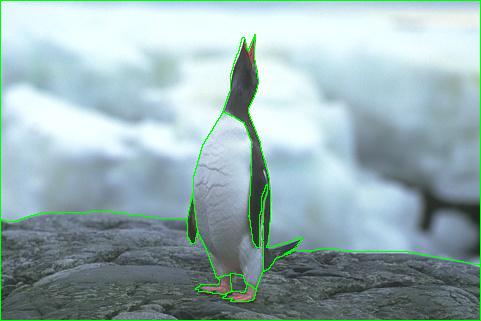
\includegraphics[scale=0.5]{images/bsd-2-ground-truth-1}
%   			\caption{Corresponding ground truth segmentation.}
%   		\end{figure}
%	\end{frame}
	
	\begin{frame}{Introduction -- Superpixels}
		\begin{figure}
   			\centering
   			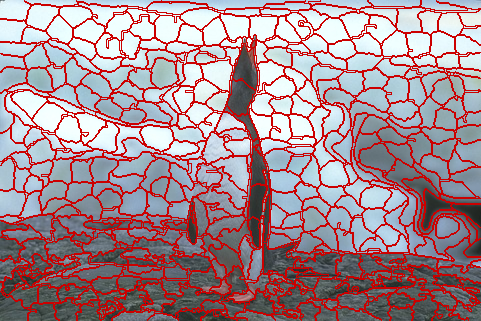
\includegraphics[scale=0.5]{images/bsd-2-reseedssm-400}
   			\caption{Example for a superpixel segmentation with exactly $400$ superpixels.}
   		\end{figure}
	\end{frame}
	
	\section{Goals}
	\begin{frame}{Goals}
		Two main goals:
		\vskip 0.25cm
		\begin{itemize}[label=1.]
			\item An analysis of using depth information for superpixel segmentation by extending the algorithm called \textbf{SEEDS} \cite{VanDenBerghBoixRoigCapitaniVanGool:2012};
		\end{itemize}
		\pause
		
		\begin{itemize}[label=2.]
			\item A thorough evaluation of several superpixel algorithms in order to provide an overview of existing approaches.
		\end{itemize}
	\end{frame}
	
	\section{Related Work}
	\begin{frame}{Related Work -- Superpixel Algorithms}
		Literature on superpixel algorithms is quite extensive.
		\vskip 0.5cm
		
		Therefore, we focus on four out of thirteen evaluated approaches:
		\vskip 0.25cm
		\begin{itemize}[leftmargin=0cm]
			\item \textbf{FH} -- Felzenswalb \& Huttenlocher \cite{FelzenswalbHuttenlocher:2004}.
			\pause
			
			\item \textbf{SLIC} -- Simple Linear Iterative Clustering \cite{AchantaShajiSmithLucchiFuaSuesstrunk:2010}.
			\pause
			
			\item \textbf{SEEDS} -- Superpixels Extracted via Energy-Driven Sampling.
			\pause
			
			\item \textbf{VCCS} -- Voxel-Cloud Connectivity Segmentation \cite{PaponAbramovSchoelerWoergoetter:2013}.
		\end{itemize}
	\end{frame}
	
	\section{SEEDS}
	\begin{frame}{SEEDS -- Idea}
		Remember:
		\vskip 0.25cm
	
		\textbf{SEEDS} refines an initial superpixel segmentation based on color histograms by:
		\vskip 0.25cm
		\begin{itemize}[label=--]
			\item Exchanging blocks of pixels between neighboring superpixels.
			\item Exchanging single pixels between neighboring superpixels.
		\end{itemize}
		\vskip 0.25cm
		
		The initial superpixel segmentation is given by a uniform grid.
	\end{frame}

%	\begin{frame}{SEEDS -- Idea}
%		\begin{figure}
%   			\centering
%   			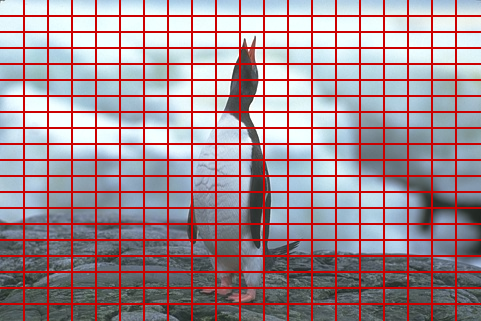
\includegraphics[scale=0.5]{images/bsd-2-level-4}
%   			\caption{Initial superpixel segmentation -- a uniform grid.}
%   		\end{figure}
%	\end{frame}

%	\begin{frame}{SEEDS -- Initialization}
%		\textbf{Initialization:}
%		\vskip 0.25cm
%		
%		\textbf{SEEDS} recursively groups pixels to form a hierarchy of $L$ levels:
%		\vskip 0.25cm
%		\begin{itemize}[label=--]
%			\item Group $w \times h$ pixels to form one block at level $l = 1$.
%			\item Group $2 \times 2$ blocks at level $(l - 1)$ to from one block at level $l > 1$.
%		\end{itemize}
%		\vskip 0.5cm
%		
%		Blocks at level $L$ are the initial superpixels.
%		\vskip 0.5cm
%		
%		\textbf{Histogram computation:}
%		\vskip 0.25cm
%		
%		Compute color histograms for each block at level $l \geq 1$.
%	\end{frame}

%	\begin{frame}{SEEDS -- Blocks and Histograms}
%		\begin{figure}
%   			\centering
%   			
\includegraphics[scale=0.5]{images/bsd-2-level-2}
%   			\caption{For $w = 3$ and $h = 2$, blocks at level $l = 2$.}
%   		\end{figure}
%	\end{frame}
%
%	\begin{frame}{SEEDS -- Blocks and Histograms}
%		\begin{figure}
%   			\centering
%   			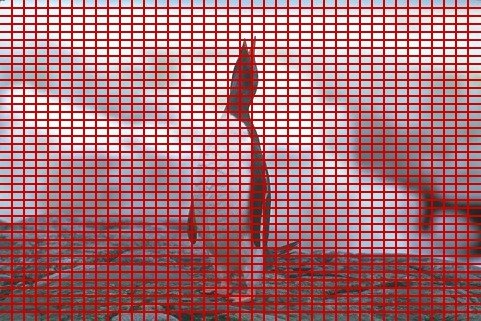
\includegraphics[scale=0.5]{images/bsd-2-level-3}
%   			\caption{For $w = 3$ and $h = 2$, blocks at level $l = 3$.}
%   		\end{figure}
%	\end{frame}

	\begin{frame}{SEEDS -- Initial Superpixels}
		\begin{figure}
   			\centering
   			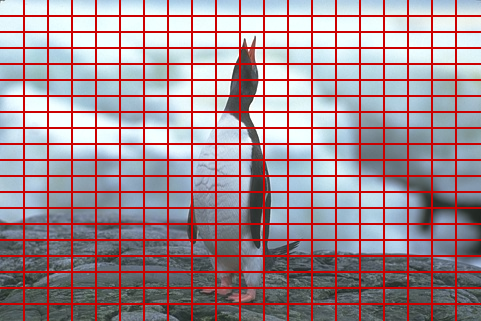
\includegraphics[scale=0.5]{images/bsd-2-level-4}
   			\caption{Initial superpixel segmentation: $400$ superpixels.}
   		\end{figure}
	\end{frame}
	
%	\begin{frame}{SEEDS -- Block Updates}
%		\textbf{Block updates:}
%		\vskip 0.25cm
%		
%		For each level $l = (L - 1)$ down to $1$:
%		\vskip 0.25cm
%		\begin{itemize}[label=--]
%			\item For each block at level $l$:
%			\vskip 0.25cm
%			\begin{itemize}[label=--]
%				\item If a neighboring block belongs to a different superpixel, consider changing the label.
%			\end{itemize}
%		\end{itemize}
%		\vskip 0.5cm
%		
%		Criterion:
%		\vskip 0.25cm
%		
%		Change the label if the intersection of block histogram and superpixel histogram is higher than before.
%		\vskip 0.25cm
%		
%		In practice: run $T$ iterations of block updates at each level.
%	\end{frame}

	\begin{frame}{SEEDS -- Block Updates}
		\begin{figure}
   			\centering
   			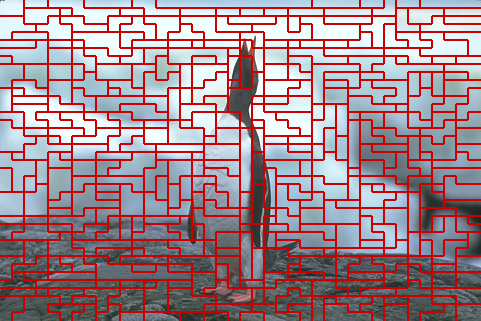
\includegraphics[scale=0.5]{images/bsd-2-after-3}
   			\caption{Superpixel segmentation after exchanging biggest blocks.}
   		\end{figure}
	\end{frame}

	\begin{frame}{SEEDS -- Block Updates}
		\begin{figure}
   			\centering
   			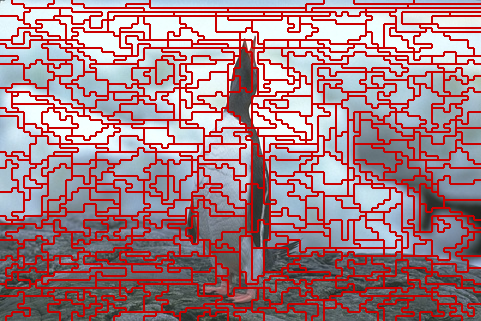
\includegraphics[scale=0.5]{images/bsd-2-after-2}
   			\caption{Superpixel segmentation after exchanging small blocks.}
   		\end{figure}
	\end{frame}
	
	\begin{frame}{SEEDS -- Block Updates}
		\begin{figure}
   			\centering
   			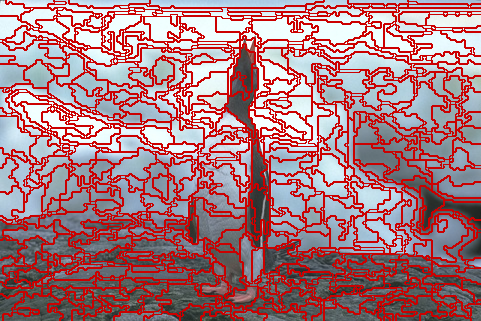
\includegraphics[scale=0.5]{images/bsd-2-after-1}
   			\caption{Superpixel segmentation after exchanging smallest blocks.}
   		\end{figure}
	\end{frame}

%	\begin{frame}{SEEDS -- Pixel Updates}
%		\textbf{Pixel updates:}
%		\vskip 0.25cm
%		
%		For each pixel:
%		\vskip 0.25cm
%		\begin{itemize}[label=--]
%			\item If a neighboring pixel belongs to a different superpixel, consider changing the label.
%		\end{itemize}
%		\vskip 0.5cm
%		
%		Two possible criteria:
%		\vskip 0.25cm
%		\begin{itemize}[label=--]
%			\item Change the label if the color of the pixel has high probability under the superpixel's color histogram.
%			\item Change the label if the color difference between pixel and superpixel is small (mean pixel updates).
%		\end{itemize}
%		
%		In practice: run $2T$ iterations of pixel updates.
%	\end{frame}
	
%	\begin{frame}{SEEDS -- Pixel Updates}
%		\begin{figure}
%   			\centering
%   			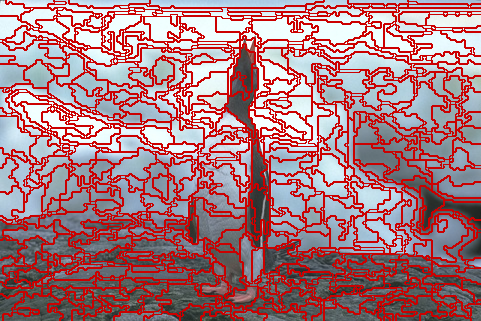
\includegraphics[scale=0.5]{images/bsd-2-after-1}
%   			\caption{Superpixel segmentation after performing block updates at level $l = 1$.}
%   		\end{figure}
%	\end{frame}
	
%	\begin{frame}{SEEDS -- Pixel Updates}
%		\begin{figure}
%   			\centering
%   			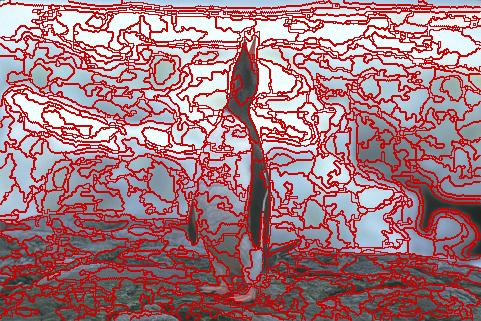
\includegraphics[scale=0.5]{images/bsd-2-reseeds-400}
%   			\caption{Superpixel segmentation generated by \textbf{SEEDS} where the pixel updates are based on color histograms.}
%   		\end{figure}
%	\end{frame}

	\begin{frame}{SEEDS -- Pixel Updates}
		\begin{figure}
   			\centering
   			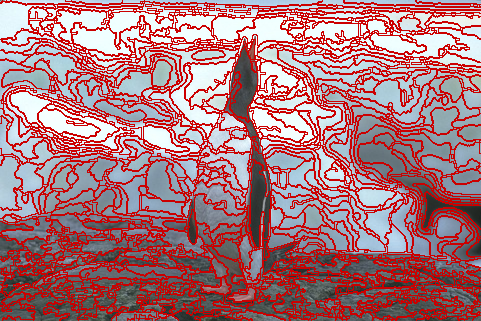
\includegraphics[scale=0.5]{images/bsd-2-reseedsmp-400}
   			\caption{Superpixel segmentation after running pixel updates.}
   		\end{figure}
	\end{frame}

	\begin{frame}{SEEDS -- Pixel Updates}
		\begin{figure}
   			\centering
   			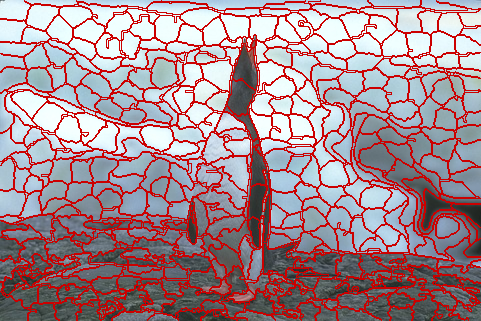
\includegraphics[scale=0.5]{images/bsd-2-reseedssm-400}
   			\caption{Superpixel segmentation after running pixel updates with an additional compactness constraint -- \textbf{SEEDS*}.}
   		\end{figure}
	\end{frame}

	\section{SEEDS with Depth}
	\begin{frame}{SEEDS -- Depth Information}
		Block updates provide a good initial superpixel segmentation for pixel updates.
		\vskip 0.5cm
	
		Goal: Integrate depth information into block updates.
		\vskip 0.25cm
		
		Ideas:
		\vskip 0.25cm
		\begin{itemize}[label=--]
			\item Depth histograms
			\item Normal histograms
			\item Mean based block updates (plane fitting)
		\end{itemize}
		\vskip 0.25cm
		\pause
		
		Unfortunately, these attempts did not result in increased performance.
		\vskip 0.25cm
	\end{frame}
	
	\begin{frame}{SEEDS -- Depth Information}
		Pixel updates seem to have the most influence on the final superpixel segmentation.
		\vskip 0.5cm
	
		Goal: Integrate depth information into pixel updates.
		\vskip 0.25cm
		
		Ideas:
		\vskip 0.25cm
		\begin{itemize}[label=--]
			\item 3D point coordinates
			\item Normal information
		\end{itemize}
		\vskip 0.5cm
	\end{frame}
	
	\begin{frame}{SEEDS -- Depth Information}
		\begin{figure}
   			\centering
   			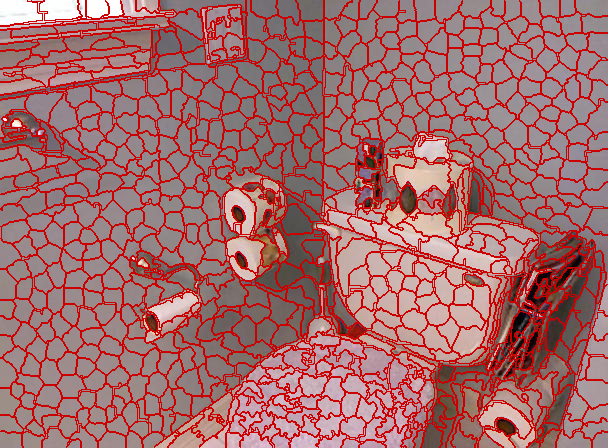
\includegraphics[scale=0.33]{images/nyu-3-reseedssm}
   			\caption{Superpixel segmentation generated by \textbf{SEEDS*}. Image taken from the NYU Depth Dataset \cite{SilbermanHoiemKohliFergus:2012}.}
   		\end{figure}
	\end{frame}
	
	\begin{frame}{SEEDS -- Depth Information}
		\begin{figure}
   			\centering
   			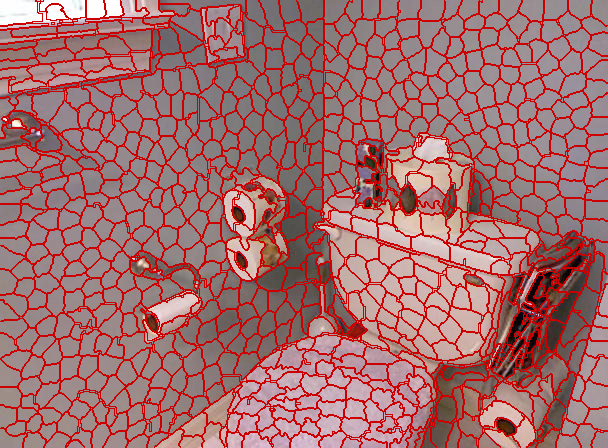
\includegraphics[scale=0.33]{images/nyu-3-seeds3d}
   			\caption{Superpixel segmentation generated by \textbf{SEEDS3D}, a variant of \textbf{SEEDS} using 3D point coordinates for pixel updates.}
   		\end{figure}
	\end{frame}
	
	\begin{frame}{SEEDS -- Depth Information}
		\begin{figure}
   			\centering
   			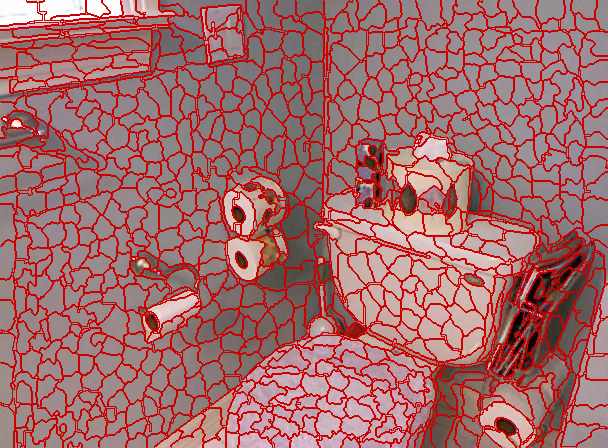
\includegraphics[scale=0.33]{images/nyu-3-seeds3dn}
   			\caption{Superpixel segmentation generated by \textbf{SEEDS3D} using normal information.}
   		\end{figure}
	\end{frame}
	
	\begin{frame}{SEEDS -- Depth Information}
		Unfortunately, few of our efforts resulted in significantly better superpixel segmentations.
		\vskip 0.5cm
		
		Possible explanations:
		\vskip 0.25cm
		\begin{itemize}[label=--]
			\item \textbf{SEEDS} performs well even without depth information -- little room for improvement.
			\pause
			
			\item Images from the NYU Depth Dataset \cite{SilbermanHoiemKohliFergus:2012} are difficult because of clutter and bad lighting.
			\begin{itemize}[label=$\rightarrow$]
				\item Noisy depth images, unreliable normal information.
			\end{itemize}
		\end{itemize}
	\end{frame}
	
	\begin{frame}{SEEDS -- Depth Information}
		\begin{figure}
   			\centering
   			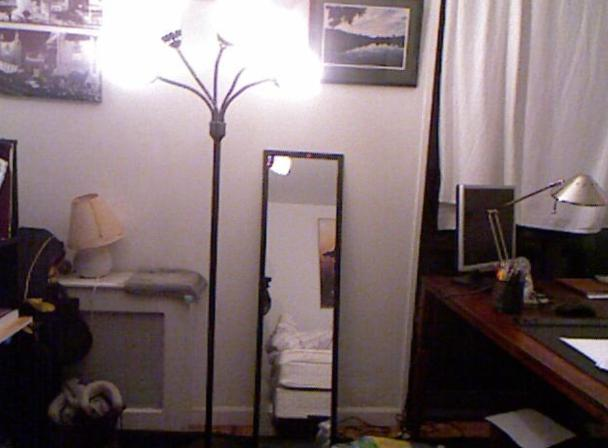
\includegraphics[scale=0.33]{images/nyu-difficult}
   			\caption{Difficult image from the NYU Depth Dataset \cite{SilbermanHoiemKohliFergus:2012}.}
   		\end{figure}
	\end{frame}
	
	\begin{frame}{SEEDS -- Depth Information}
		\begin{figure}
   			\centering
   			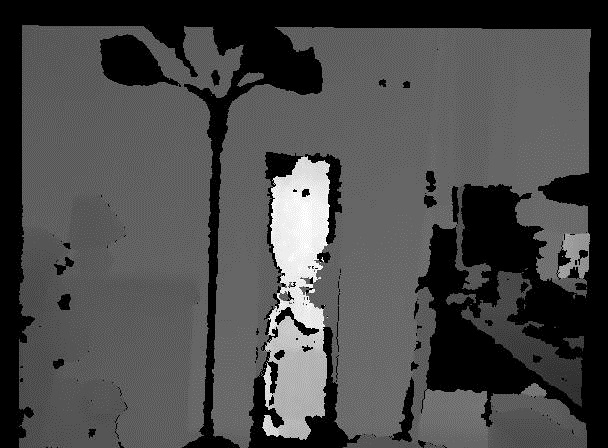
\includegraphics[scale=0.439]{images/nyu-difficult-raw-depth}
   			\caption{Corresponding raw depth image.}
   		\end{figure}
	\end{frame}
	
	\begin{frame}{SEEDS -- Depth Information}
		\begin{figure}
   			\centering
   			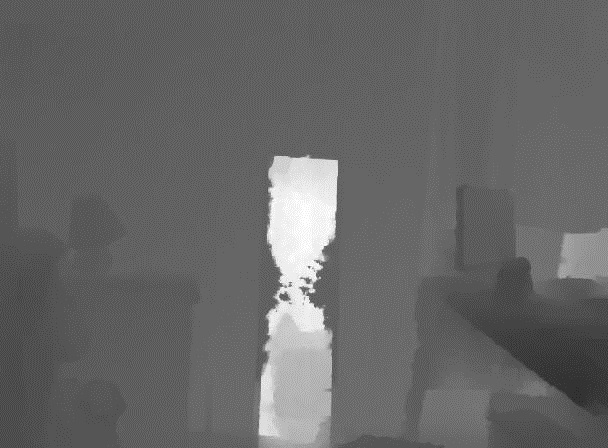
\includegraphics[scale=0.439]{images/nyu-difficult-depth}
   			\caption{Pre-processed depth image.}
   		\end{figure}
	\end{frame}
	
	\begin{frame}{SEEDS -- Depth Information}
		\begin{figure}
   			\centering
   			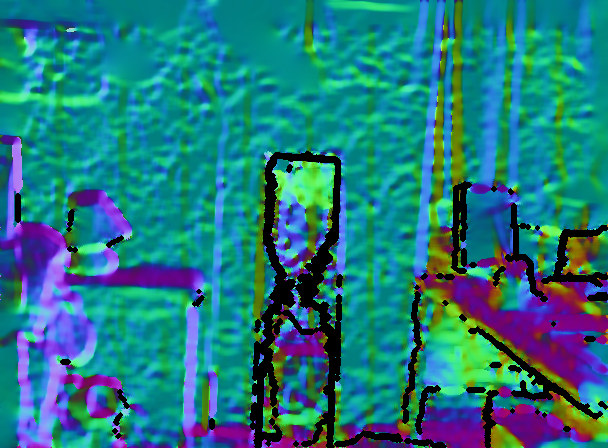
\includegraphics[scale=0.33]{images/nyu-difficult-normal}
   			\caption{Computed normals (color coded) using the Point Cloud Library \cite{RusuCousins:2011}.}
   		\end{figure}
	\end{frame}
	
	\section{Evaluation}
	\begin{frame}{Evaluation}
		Remember, the algorithms:
		\vskip 0.25cm
		\begin{itemize}[leftmargin=0cm]
			\item \textbf{FH} -- Felzenswalb \& Huttenlocher \cite{FelzenswalbHuttenlocher:2004}.
			\item \textbf{SLIC} -- Simple Linear Iterative Clustering \cite{AchantaShajiSmithLucchiFuaSuesstrunk:2010}.
			\item \textbf{SEEDS} -- Superpixels Extracted via Energy-Driven Sampling.
			\item \textbf{VCCS} -- Voxel-Cloud Connectivity Segmentation \cite{PaponAbramovSchoelerWoergoetter:2013}.
		\end{itemize}
	\end{frame}
	
	\begin{frame}{Evaluation}
		Used datasets:
		\vskip 0.25cm
		\begin{itemize}[label=--]
			\item Berkeley Segmentation Dataset (BSDS500) \cite{ArbelaezMaireFowlkesMalik:2011}: 500 natural images.
			\item NYU Depth Dataset (NYUV2) \cite{SilbermanHoiemKohliFergus:2012}: 1449 images of indoor scenes with depth information.
		\end{itemize}
		
		\begin{figure}
			\subfigure{
				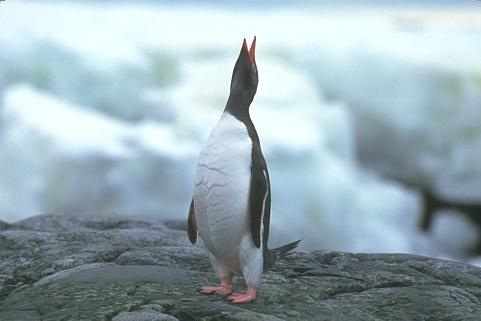
\includegraphics[scale=0.1675]{images/bsd-2}
			}
			\subfigure{
				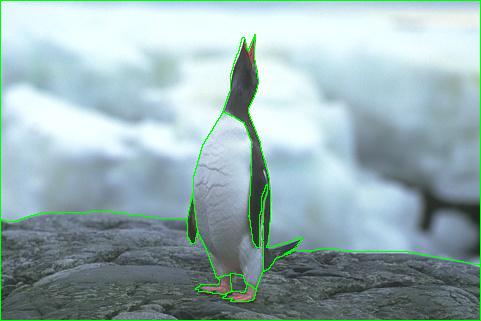
\includegraphics[scale=0.1675]{images/bsd-2-ground-truth-1}
			}
			\subfigure{
				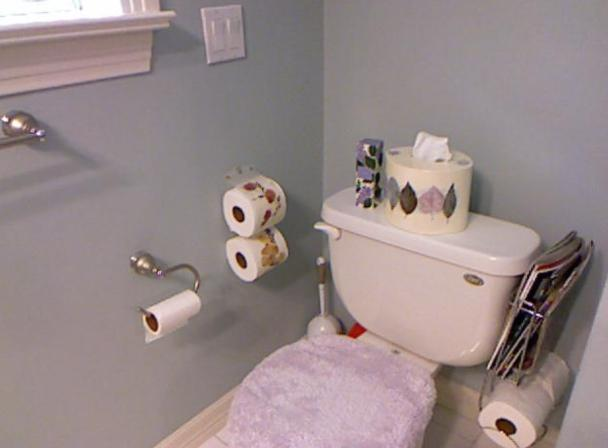
\includegraphics[scale=0.12]{images/nyu-3}
			}
			\subfigure{
				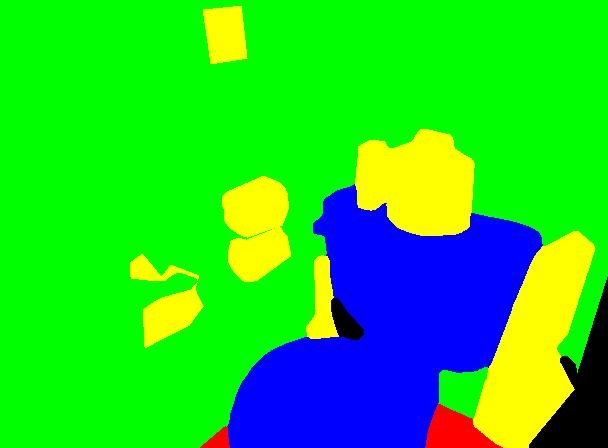
\includegraphics[scale=0.16]{images/nyu-3-labels}
			}
			\caption{Images and corresponding ground truth segmentations from the BSDS500 and the NYUV2.}
		\end{figure}
	\end{frame}
	
	\begin{frame}{Evaluation}
	
		Parameters have been optimized on training sets with respect to:
		\vskip 0.25cm
		
		\begin{itemize}[label=--]
			\item Boundary Recall $Rec$: the fraction of boundary pixels in the ground truth segmentation correctly detected in the superpixel segmentation.
			\vskip 0.25cm
			\begin{itemize}[label=$\rightarrow$]
				\item $100\%$ is best.
			\end{itemize}
			\vskip 0.25cm
			\pause
			
			\item Undersegmentation Error $UE$: the error made when comparing the ground truth segmentation to the superpixel segmentation.
			\vskip 0.25cm
			\begin{itemize}[label=$\rightarrow$]
				\item $0\%$ is best.
			\end{itemize}
		\end{itemize}
		\vskip 0.25cm
		\pause
		
		Qualitative and quantitative comparison on test sets.
	\end{frame}
	
	\subsection{Qualitative}
%	\begin{frame}{Qualitative Comparison}
%		Qualitative comparison:
%		\vskip 0.25cm
%		\begin{itemize}[label=--]
%			\item Compactness
%			\item Regularity
%		\end{itemize}
%		\vskip 0.25cm
%		
%		Compact and regular superpixels are regarded as visually appealing.
%		\vskip 0.5cm
%		\pause
%		
%		Remember: Parameters have been chosen in order to optimize Boundary Recall and Undersegmentation Error.
%		\vskip 0.25cm
%		
%		\textbf{oriSEEDS}: original implementation of \textbf{SEEDS}.
%		\vskip 0.25cm
%		
%		\textbf{reSEEDS}: our implementation of \textbf{SEEDS}.
%	\end{frame}
	
	\begin{frame}{Qualitative Comparison -- FH}
		\begin{figure}
   			\centering
   			\subfigure{
   				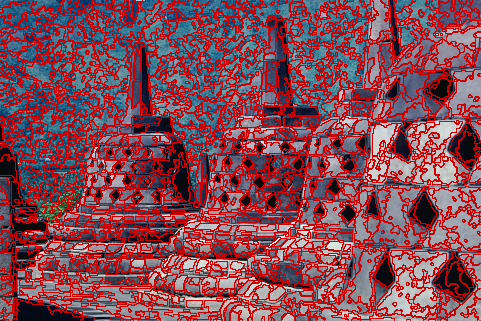
\includegraphics[scale=0.3475]{images/bsd-test-1-fh}
   			}
   			\subfigure{
   				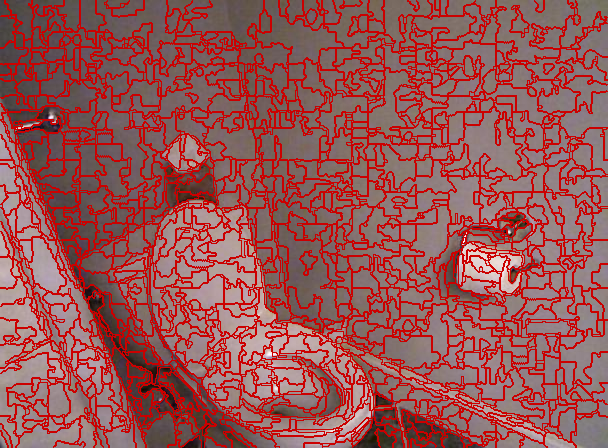
\includegraphics[scale=0.25]{images/nyu-test-3-fh}
   			}
   			\caption{Superpixel segmentations generated by \textbf{FH}.}
   		\end{figure}
	\end{frame}
	
	\begin{frame}{Qualitative Comparison -- SLIC}
		\begin{figure}
   			\centering
   			\subfigure{
   				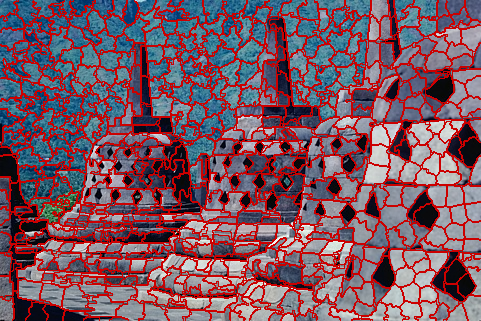
\includegraphics[scale=0.3475]{images/bsd-test-1-orislic}
   			}
   			\subfigure{
   				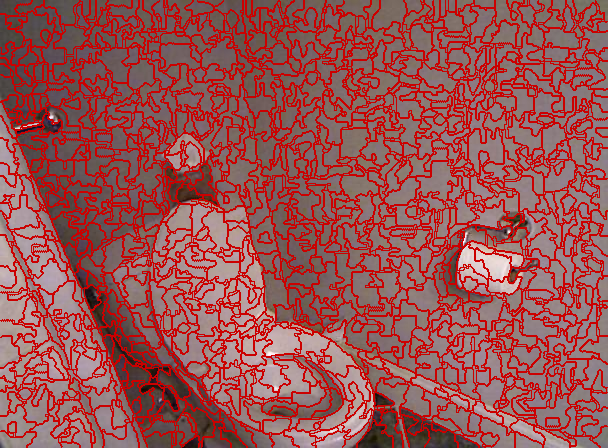
\includegraphics[scale=0.25]{images/nyu-test-3-orislic}
   			}
   			\caption{Superpixel segmentations generated by \textbf{SLIC}.}
   		\end{figure}
	\end{frame}
	
	\begin{frame}{Qualitative Comparison -- oriSEEDS}
		\begin{figure}
   			\centering
   			\subfigure{
   				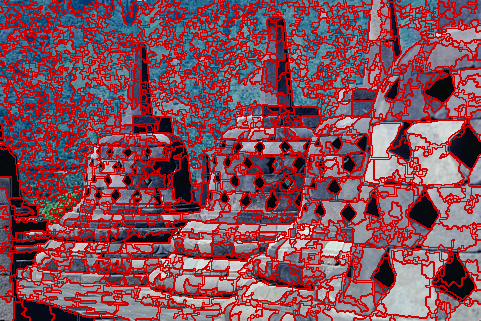
\includegraphics[scale=0.3475]{images/bsd-test-1-oriseedsmp}
   			}
   			\subfigure{
   				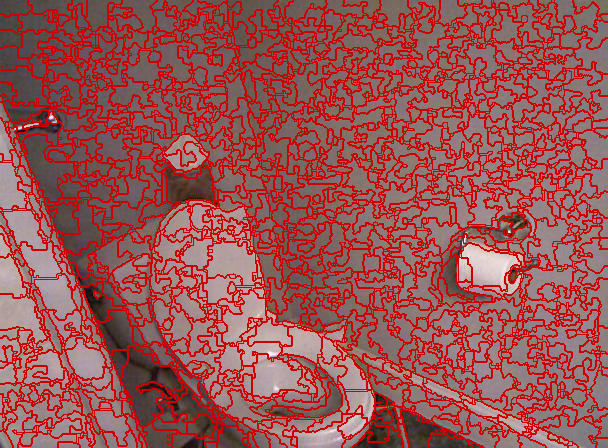
\includegraphics[scale=0.25]{images/nyu-test-3-oriseedsmp}
   			}
   			\caption{Superpixel segmentations generated by \textbf{oriSEEDS}.}
   		\end{figure}
	\end{frame}
	
	\begin{frame}{Qualitative Comparison -- reSEEDS*}
		\begin{figure}
   			\centering
   			\subfigure{
   				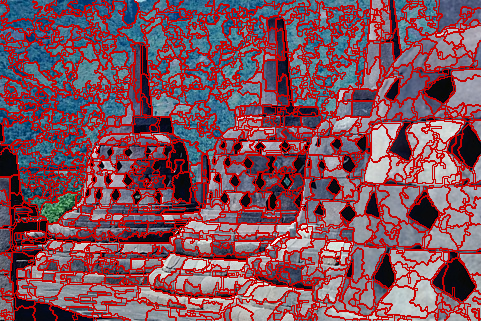
\includegraphics[scale=0.3475]{images/bsd-test-1-reseedssm}
   			}
   			\subfigure{
   				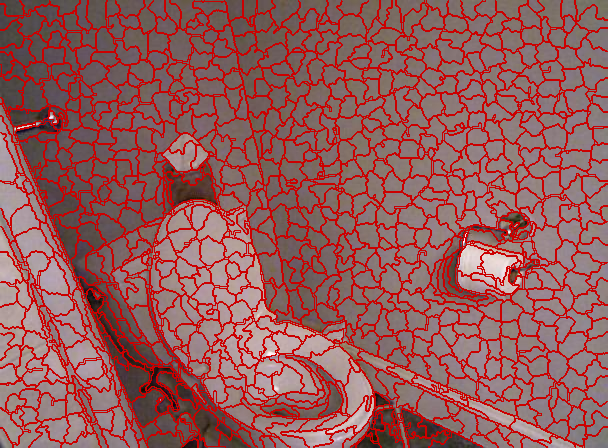
\includegraphics[scale=0.25]{images/nyu-test-3-reseedssm}
   			}
   			\caption{Superpixel segmentations generated by \textbf{reSEEDS*}.}
   		\end{figure}
	\end{frame}
	
	\begin{frame}{Qualitative Comparison -- SEEDS3D}
		\begin{figure}
   			\centering
   			\subfigure{
   				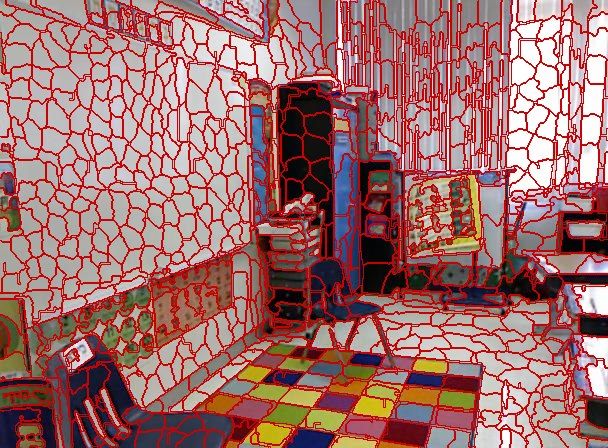
\includegraphics[scale=0.25]{images/nyu-test-5-seeds3d}
   			}
   			\subfigure{
   				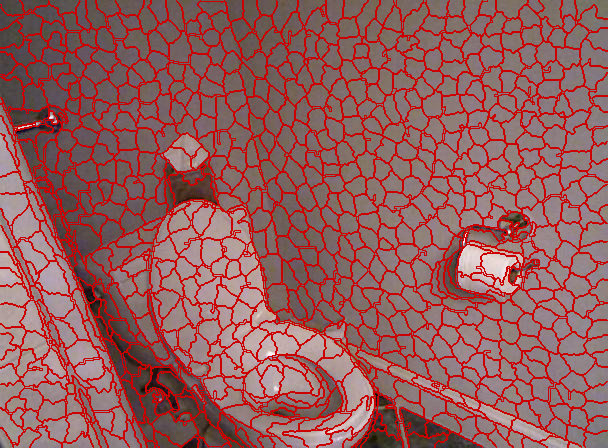
\includegraphics[scale=0.25]{images/nyu-test-3-seeds3d}
   			}
   			\caption{Superpixel segmentations generated by \textbf{SEEDS3D}.}
   		\end{figure}
	\end{frame}
	
	\begin{frame}{Qualitative Comparison -- VCCS}
		\begin{figure}
   			\centering
   			\subfigure{
   				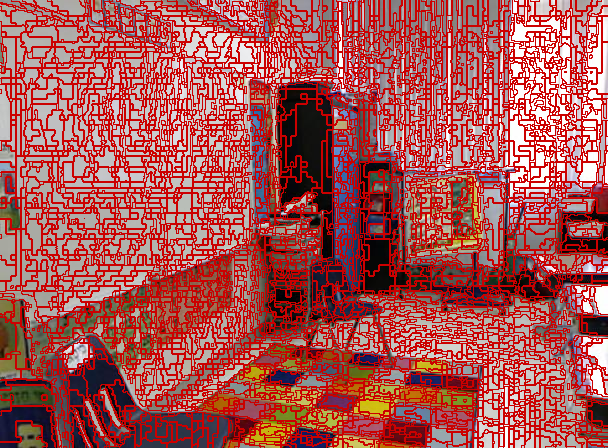
\includegraphics[scale=0.25]{images/nyu-test-5-vccs}
   			}
   			\subfigure{
   				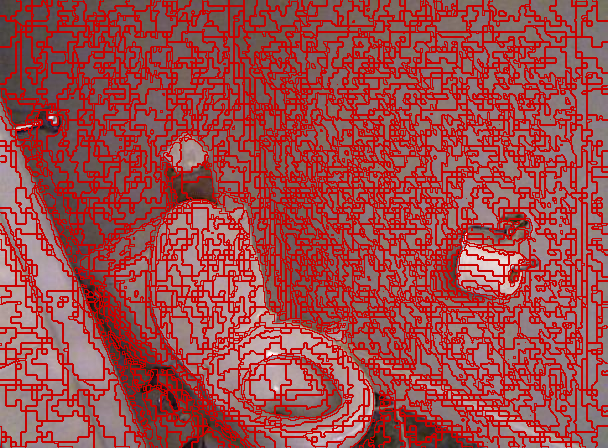
\includegraphics[scale=0.25]{images/nyu-test-3-vccs}
   			}
   			\caption{Superpixel segmentations generated by \textbf{VCCS}.}
   		\end{figure}
	\end{frame}
	
%	\begin{frame}{Qualitative Comparison -- Conclusion}
%		Observation: Superpixels are neither very compact nor regular for most of the algorithms.
%		\vskip 0.5cm
%		
%		Remark:
%		\vskip 0.25cm
%		\begin{itemize}[label=--]
%			\item Some algorithms offer control over the compactness: \textbf{SLIC}, \textbf{reSEEDS*} and \textbf{VCCS}.
%			\vskip 0.25cm
%			\begin{itemize}[label=$\rightarrow$]
%				\item Allows to trade performance for compactness and vice versa.
%			\end{itemize}
%		\end{itemize}
%	\end{frame}

	\subsection{Quantitative}
% ==================================================================
% \/ quantitative comparison BSDS500
	\begin{frame}{Quantitative Comparison -- BSDS500}
		\vspace{-0.5cm}
		\begin{figure}
			\centering
			\subfigure{
				\begin{tikzpicture}
					\begin{axis}[
						height=7cm,
						width=4cm,
						xlabel=Superpixels,
						ylabel=$Rec$,
						ymin=0.9,
						ymax=1,
						xmin=100,
						xmax=1200,
						cycle list name=comparison bsd 1]
				
						% oriSEEDSmp
						\addplot+[thick] table [row sep=newline,trim cells=true,x=K,y=Rec] {data/oriseedsmp-bsd-test.csv};	
						\label{plot:evaluation-comparison-oriseedsmp-rec-bsd}
					
						% reSEEDSmp*
						\addplot+[thick] table [row sep=newline,trim cells=true,x=K,y=Rec] {data/reseedssm-bsd-test.csv};
						\label{plot:evaluation-comparison-reseedssm-rec-bsd}
					
					\end{axis}
				\end{tikzpicture}
			}
			\subfigure{
				\begin{tikzpicture}
					\begin{axis}[
						height=7cm,
						width=4cm,
						xlabel=Superpixels,
						ylabel=$UE$,
						ymin=0.03,
						ymax=0.1,
						ytick={0.03,0.04,0.06,0.08,0.1},
						xmin=100,
						xmax=1200,
						cycle list name=comparison bsd 1]
					
						% oriSEEDSmp
						\addplot+[thick] table [row sep=newline,trim cells=true,x=K,y=UE] {data/oriseedsmp-bsd-test.csv};	
						\label{plot:evaluation-comparison-oriseedsmp-ue-bsd}
					
						% reSEEDSmp*
						\addplot+[thick] table [row sep=newline,trim cells=true,x=K,y=UE] {data/reseedssm-bsd-test.csv};
						\label{plot:evaluation-comparison-reseedssm-ue-bsd}
					
					\end{axis}
					\matrix[%
							matrix of nodes,%
							anchor=north west,%
							inner sep=0.25em,%
							nodes={font=\small},%
							column 1/.append style={anchor=base west},%
						] at ($(current axis.north east) + (0.25,0)$) {
							BSDS500:\\
							\ref{plot:evaluation-comparison-oriseedsmp-ue-bsd} \textbf{oriSEEDS}\\
							\ref{plot:evaluation-comparison-reseedssm-ue-bsd} \textbf{reSEEDS*}\\
						};
				\end{tikzpicture}
			}
		\end{figure}
	\end{frame}
	
	\begin{frame}{Quantitative Comparison -- BSDS500}
		\vspace{-0.5cm}
		\begin{figure}
			\centering
			\subfigure{
				\begin{tikzpicture}
					\begin{axis}[
						height=7cm,
						width=4cm,
						xlabel=Superpixels,
						ylabel=$Rec$,
						ymin=0.9,
						ymax=1,
						xmin=100,
						xmax=1200,
						cycle list name=comparison bsd 2]
					
						% SLIC
						\addplot+[thick] table [row sep=newline,trim cells=true,x=K,y=Rec] {data/orislic-bsd-test.csv};
						\label{plot:evaluation-comparison-orislic-rec-bsd}
					
						% oriSEEDSmp
						\addplot+[thick] table [row sep=newline,trim cells=true,x=K,y=Rec] {data/oriseedsmp-bsd-test.csv};	
						\label{plot:evaluation-comparison-oriseedsmp-rec-bsd}
					
						% reSEEDSmp*
						\addplot+[thick] table [row sep=newline,trim cells=true,x=K,y=Rec] {data/reseedssm-bsd-test.csv};
						\label{plot:evaluation-comparison-reseedssm-rec-bsd}
					
					\end{axis}
				\end{tikzpicture}
			}
			\subfigure{
				\begin{tikzpicture}
					\begin{axis}[
						height=7cm,
						width=4cm,
						xlabel=Superpixels,
						ylabel=$UE$,
						ymin=0.03,
						ymax=0.1,
						ytick={0.03,0.04,0.06,0.08,0.1},
						xmin=100,
						xmax=1200,
						cycle list name=comparison bsd 2]
					
						% SLIC
						\addplot+[thick] table [row sep=newline,trim cells=true,x=K,y=UE] {data/orislic-bsd-test.csv};
						\label{plot:evaluation-comparison-orislic-ue-bsd}
					
						% oriSEEDSmp
						\addplot+[thick] table [row sep=newline,trim cells=true,x=K,y=UE] {data/oriseedsmp-bsd-test.csv};	
						\label{plot:evaluation-comparison-oriseedsmp-ue-bsd}
					
						% reSEEDSmp*
						\addplot+[thick] table [row sep=newline,trim cells=true,x=K,y=UE] {data/reseedssm-bsd-test.csv};
						\label{plot:evaluation-comparison-reseedssm-ue-bsd}
					
					\end{axis}
					\matrix[%
							matrix of nodes,%
							anchor=north west,%
							inner sep=0.25em,%
							nodes={font=\small},%
							column 1/.append style={anchor=base west},%
						] at ($(current axis.north east) + (0.25,0)$) {
							BSDS500:\\
							\ref{plot:evaluation-comparison-orislic-ue-bsd} \textbf{SLIC}\\
							\ref{plot:evaluation-comparison-oriseedsmp-ue-bsd} \textbf{oriSEEDS}\\
							\ref{plot:evaluation-comparison-reseedssm-ue-bsd} \textbf{reSEEDS*}\\
						};
				\end{tikzpicture}
			}
		\end{figure}
	\end{frame}
	
	\begin{frame}{Quantitative Comparison -- BSDS500}
		\vspace{-0.5cm}
		\begin{figure}
			\centering
			\subfigure{
				\begin{tikzpicture}
					\begin{axis}[
						height=7cm,
						width=4cm,
						xlabel=Superpixels,
						ylabel=$Rec$,
						ymin=0.9,
						ymax=1,
						xmin=100,
						xmax=1200,
						cycle list name=comparison bsd 3]
				
						% FH
						\addplot+[thick] table [row sep=newline,trim cells=true,x=K,y=Rec] {data/fh-bsd-test.csv};
						\label{plot:evaluation-comparison-fh-rec-bsd}
					
						% SLIC
						\addplot+[thick] table [row sep=newline,trim cells=true,x=K,y=Rec] {data/orislic-bsd-test.csv};
						\label{plot:evaluation-comparison-orislic-rec-bsd}
					
						% oriSEEDSmp
						\addplot+[thick] table [row sep=newline,trim cells=true,x=K,y=Rec] {data/oriseedsmp-bsd-test.csv};	
						\label{plot:evaluation-comparison-oriseedsmp-rec-bsd}
					
						% reSEEDSmp*
						\addplot+[thick] table [row sep=newline,trim cells=true,x=K,y=Rec] {data/reseedssm-bsd-test.csv};
						\label{plot:evaluation-comparison-reseedssm-rec-bsd}
					
					\end{axis}
				\end{tikzpicture}
			}
			\subfigure{
				\begin{tikzpicture}
					\begin{axis}[
						height=7cm,
						width=4cm,
						xlabel=Superpixels,
						ylabel=$UE$,
						ymin=0.03,
						ymax=0.1,
						ytick={0.03,0.04,0.06,0.08,0.1},
						xmin=100,
						xmax=1200,
						cycle list name=comparison bsd 3]
					
						% FH
						\addplot+[thick] table [row sep=newline,trim cells=true,x=K,y=UE] {data/fh-bsd-test.csv};
						\label{plot:evaluation-comparison-fh-ue-bsd}
					
						% SLIC
						\addplot+[thick] table [row sep=newline,trim cells=true,x=K,y=UE] {data/orislic-bsd-test.csv};
						\label{plot:evaluation-comparison-orislic-ue-bsd}
					
						% oriSEEDSmp
						\addplot+[thick] table [row sep=newline,trim cells=true,x=K,y=UE] {data/oriseedsmp-bsd-test.csv};	
						\label{plot:evaluation-comparison-oriseedsmp-ue-bsd}
					
						% reSEEDSmp*
						\addplot+[thick] table [row sep=newline,trim cells=true,x=K,y=UE] {data/reseedssm-bsd-test.csv};
						\label{plot:evaluation-comparison-reseedssm-ue-bsd}
					
					\end{axis}
					\matrix[%
							matrix of nodes,%
							anchor=north west,%
							inner sep=0.25em,%
							nodes={font=\small},%
							column 1/.append style={anchor=base west},%
						] at ($(current axis.north east) + (0.25,0)$) {
							BSDS500:\\
							\ref{plot:evaluation-comparison-fh-ue-bsd} \textbf{FH}\\
							\ref{plot:evaluation-comparison-orislic-ue-bsd} \textbf{SLIC}\\
							\ref{plot:evaluation-comparison-oriseedsmp-ue-bsd} \textbf{oriSEEDS}\\
							\ref{plot:evaluation-comparison-reseedssm-ue-bsd} \textbf{reSEEDS*}\\
						};
				\end{tikzpicture}
			}
		\end{figure}
	\end{frame}
	
% ==================================================================
% \/ quantitative comparison NYUV2
	\begin{frame}{Quantitative Comparison -- NYUV2}
		\vspace{-0.5cm}
		\begin{figure}
			\centering
			\subfigure{
				\begin{tikzpicture}
					\begin{axis}[
						height=7cm,
						width=4cm,
						xlabel=Superpixels,
						ylabel=$Rec$,
						ymin=0.91,
						ymax=1,
						ytick={0.91,0.92,0.94,0.96,0.98,1},
						xmin=300,
						xmax=1700,
						cycle list name=comparison nyu 1]
					
						% oriSEEDSmp
						\addplot+[thick] table [row sep=newline,trim cells=true,x=K,y=Rec] {data/oriseedsmp-nyu-test.csv};	
						\label{plot:evaluation-comparison-oriseedsmp-rec-nyu}
					
						% reSEEDSmp*
						\addplot+[thick] table [row sep=newline,trim cells=true,x=K,y=Rec] {data/reseedssm-nyu-test.csv};
						\label{plot:evaluation-comparison-reseedssm-rec-nyu}
					
						% SEEDS3D
						\addplot+[thick] table [row sep=newline,trim cells=true,x=K,y=Rec] {data/seeds3d-nyu-test.csv};
						\label{plot:evaluation-comparison-seeds3d-rec-nyu}
					
					\end{axis}
				\end{tikzpicture}
			}
			\subfigure{
				\begin{tikzpicture}
					\begin{axis}[
						height=7cm,
						width=4cm,
						xlabel=Superpixels,
						ylabel=$UE$,
						ymin=0.07,
						ymax=0.19,
						ytick={0.07,0.08,0.1,0.12,0.14,0.16,0.18,0.19},
						xmin=300,
						xmax=1700,
						cycle list name=comparison nyu 1]
					
						% oriSEEDSmp
						\addplot+[thick] table [row sep=newline,trim cells=true,x=K,y=UE] {data/oriseedsmp-nyu-test.csv};	
						\label{plot:evaluation-comparison-oriseedsmp-ue-nyu}
					
						% reSEEDSmp*
						\addplot+[thick] table [row sep=newline,trim cells=true,x=K,y=UE] {data/reseedssm-nyu-test.csv};
						\label{plot:evaluation-comparison-reseedssm-ue-nyu}
					
						% SEEDS3D
						\addplot+[thick] table [row sep=newline,trim cells=true,x=K,y=UE] {data/seeds3d-nyu-test.csv};
						\label{plot:evaluation-comparison-seeds3d-ue-nyu}
					
					\end{axis}
					\matrix[%
							matrix of nodes,%
							anchor=north west,%
							inner sep=0.25em,%
							nodes={font=\small},%
							column 1/.append style={anchor=base west},%
						] at ($(current axis.north east) + (0.25,0)$) {
							NYUV2:\\
							\ref{plot:evaluation-comparison-oriseedsmp-ue-nyu} \textbf{oriSEEDS}\\
							\ref{plot:evaluation-comparison-reseedssm-ue-nyu} \textbf{reSEEDS*}\\
							\ref{plot:evaluation-comparison-seeds3d-ue-nyu} \textbf{SEEDS3D}\\
						};
				\end{tikzpicture}
			}
		\end{figure}
	\end{frame}
	
	\begin{frame}{Quantitative Comparison -- NYUV2}
		\vspace{-0.5cm}
		\begin{figure}
			\centering
			\subfigure{
				\begin{tikzpicture}
					\begin{axis}[
						height=7cm,
						width=4cm,
						xlabel=Superpixels,
						ylabel=$Rec$,
						ymin=0.91,
						ymax=1,
						ytick={0.91,0.92,0.94,0.96,0.98,1},
						xmin=300,
						xmax=1700,
						cycle list name=comparison nyu 2]
					
						% FH
						\addplot+[thick] table [row sep=newline,trim cells=true,x=K,y=Rec] {data/fh-nyu-test.csv};
						\label{plot:evaluation-comparison-fh-rec-nyu}
					
						% SLIC
						\addplot+[thick] table [row sep=newline,trim cells=true,x=K,y=Rec] {data/orislic-nyu-test.csv};
						\label{plot:evaluation-comparison-orislic-rec-nyu}
					
						% oriSEEDSmp
						\addplot+[thick] table [row sep=newline,trim cells=true,x=K,y=Rec] {data/oriseedsmp-nyu-test.csv};	
						\label{plot:evaluation-comparison-oriseedsmp-rec-nyu}
					
						% reSEEDSmp*
						\addplot+[thick] table [row sep=newline,trim cells=true,x=K,y=Rec] {data/reseedssm-nyu-test.csv};
						\label{plot:evaluation-comparison-reseedssm-rec-nyu}
					
						% SEEDS3D
						\addplot+[thick] table [row sep=newline,trim cells=true,x=K,y=Rec] {data/seeds3d-nyu-test.csv};
						\label{plot:evaluation-comparison-seeds3d-rec-nyu}
					
					\end{axis}
				\end{tikzpicture}
			}
			\subfigure{
				\begin{tikzpicture}
					\begin{axis}[
						height=7cm,
						width=4cm,
						xlabel=Superpixels,
						ylabel=$UE$,
						ymin=0.07,
						ymax=0.19,
						ytick={0.07,0.08,0.1,0.12,0.14,0.16,0.18,0.19},
						xmin=300,
						xmax=1700,
						cycle list name=comparison nyu 2]
					
						% FH
						\addplot+[thick] table [row sep=newline,trim cells=true,x=K,y=UE] {data/fh-nyu-test.csv};
						\label{plot:evaluation-comparison-fh-ue-nyu}
					
						% SLIC
						\addplot+[thick] table [row sep=newline,trim cells=true,x=K,y=UE] {data/orislic-nyu-test.csv};
						\label{plot:evaluation-comparison-orislic-ue-nyu}
					
						% oriSEEDSmp
						\addplot+[thick] table [row sep=newline,trim cells=true,x=K,y=UE] {data/oriseedsmp-nyu-test.csv};	
						\label{plot:evaluation-comparison-oriseedsmp-ue-nyu}
					
						% reSEEDSmp*
						\addplot+[thick] table [row sep=newline,trim cells=true,x=K,y=UE] {data/reseedssm-nyu-test.csv};
						\label{plot:evaluation-comparison-reseedssm-ue-nyu}
					
						% SEEDS3D
						\addplot+[thick] table [row sep=newline,trim cells=true,x=K,y=UE] {data/seeds3d-nyu-test.csv};
						\label{plot:evaluation-comparison-seeds3d-ue-nyu}
					
					\end{axis}
					\matrix[%
							matrix of nodes,%
							anchor=north west,%
							inner sep=0.25em,%
							nodes={font=\small},%
							column 1/.append style={anchor=base west},%
						] at ($(current axis.north east) + (0.25,0)$) {
							NYUV2:\\
							\ref{plot:evaluation-comparison-fh-ue-nyu} \textbf{FH}\\
							\ref{plot:evaluation-comparison-orislic-ue-nyu} \textbf{SLIC}\\
							\ref{plot:evaluation-comparison-oriseedsmp-ue-nyu} \textbf{oriSEEDS}\\
							\ref{plot:evaluation-comparison-reseedssm-ue-nyu} \textbf{reSEEDS*}\\
							\ref{plot:evaluation-comparison-seeds3d-ue-nyu} \textbf{SEEDS3D}\\
						};
				\end{tikzpicture}
			}
		\end{figure}
	\end{frame}
	
	\begin{frame}{Quantitative Comparison -- NYUV2}
		\vspace{-0.5cm}
		\begin{figure}
			\centering
			\subfigure{
				\begin{tikzpicture}
					\begin{axis}[
						height=7cm,
						width=4cm,
						xlabel=Superpixels,
						ylabel=$Rec$,
						ymin=0.91,
						ymax=1,
						ytick={0.91,0.92,0.94,0.96,0.98,1},
						xmin=300,
						xmax=1700,
						cycle list name=comparison nyu 3]
					
						% FH
						\addplot+[thick] table [row sep=newline,trim cells=true,x=K,y=Rec] {data/fh-nyu-test.csv};
						\label{plot:evaluation-comparison-fh-rec-nyu}
					
						% SLIC
						\addplot+[thick] table [row sep=newline,trim cells=true,x=K,y=Rec] {data/orislic-nyu-test.csv};
						\label{plot:evaluation-comparison-orislic-rec-nyu}
					
						% oriSEEDSmp
						\addplot+[thick] table [row sep=newline,trim cells=true,x=K,y=Rec] {data/oriseedsmp-nyu-test.csv};	
						\label{plot:evaluation-comparison-oriseedsmp-rec-nyu}
					
						% reSEEDSmp*
						\addplot+[thick] table [row sep=newline,trim cells=true,x=K,y=Rec] {data/reseedssm-nyu-test.csv};
						\label{plot:evaluation-comparison-reseedssm-rec-nyu}
					
						% SEEDS3D
						\addplot+[thick] table [row sep=newline,trim cells=true,x=K,y=Rec] {data/seeds3d-nyu-test.csv};
						\label{plot:evaluation-comparison-seeds3d-rec-nyu}
					
						% VCCS
						\addplot+[thick] table [row sep=newline,trim cells=true,x=K,y=Rec] {data/vccs-depth-test.csv};
						\label{plot:evaluation-comparison-vccs-rec-nyu}
					
					\end{axis}
				\end{tikzpicture}
			}
			\subfigure{
				\begin{tikzpicture}
					\begin{axis}[
						height=7cm,
						width=4cm,
						xlabel=Superpixels,
						ylabel=$UE$,
						ymin=0.07,
						ymax=0.19,
						ytick={0.07,0.08,0.1,0.12,0.14,0.16,0.18,0.19},
						xmin=300,
						xmax=1700,
						cycle list name=comparison nyu 3]
					
						% FH
						\addplot+[thick] table [row sep=newline,trim cells=true,x=K,y=UE] {data/fh-nyu-test.csv};
						\label{plot:evaluation-comparison-fh-ue-nyu}
					
						% SLIC
						\addplot+[thick] table [row sep=newline,trim cells=true,x=K,y=UE] {data/orislic-nyu-test.csv};
						\label{plot:evaluation-comparison-orislic-ue-nyu}
					
						% oriSEEDSmp
						\addplot+[thick] table [row sep=newline,trim cells=true,x=K,y=UE] {data/oriseedsmp-nyu-test.csv};	
						\label{plot:evaluation-comparison-oriseedsmp-ue-nyu}
					
						% reSEEDSmp*
						\addplot+[thick] table [row sep=newline,trim cells=true,x=K,y=UE] {data/reseedssm-nyu-test.csv};
						\label{plot:evaluation-comparison-reseedssm-ue-nyu}
					
						% SEEDS3D
						\addplot+[thick] table [row sep=newline,trim cells=true,x=K,y=UE] {data/seeds3d-nyu-test.csv};
						\label{plot:evaluation-comparison-seeds3d-ue-nyu}
					
						% VCCS
						\addplot+[thick] table [row sep=newline,trim cells=true,x=K,y=UE] {data/vccs-depth-test.csv};
						\label{plot:evaluation-comparison-vccs-ue-nyu}
					
					\end{axis}
					\matrix[%
							matrix of nodes,%
							anchor=north west,%
							inner sep=0.25em,%
							nodes={font=\small},%
							column 1/.append style={anchor=base west},%
						] at ($(current axis.north east) + (0.25,0)$) {
							NYUV2:\\
							\ref{plot:evaluation-comparison-fh-ue-nyu} \textbf{FH}\\
							\ref{plot:evaluation-comparison-orislic-ue-nyu} \textbf{SLIC}\\
							\ref{plot:evaluation-comparison-oriseedsmp-ue-nyu} \textbf{oriSEEDS}\\
							\ref{plot:evaluation-comparison-reseedssm-ue-nyu} \textbf{reSEEDS*}\\
							\ref{plot:evaluation-comparison-seeds3d-ue-nyu} \textbf{SEEDS3D}\\
							\ref{plot:evaluation-comparison-vccs-ue-nyu} \textbf{VCCS}\\
						};
				\end{tikzpicture}
			}
		\end{figure}
	\end{frame}
	
%	\begin{frame}{Quantitative Comparison -- Discussion}
%		\textbf{FH} performs excellent on both datasets, only outperformed by \textbf{VCCS}.
%		\vskip 0.25cm
%		\begin{itemize}[label=--]
%			\item However, \textbf{FH} does not offer control over the number of superpixels.
%			\vskip 0.25cm
%			\begin{itemize}[label=$\rightarrow$]
%				\item In practice, difficult to choose parameters.
%			\end{itemize}
%			\item \textbf{VCCS} operates on a point cloud.
%		\end{itemize}
%		\vskip 0.5cm
%		\pause
%		
%		Our implementation of \textbf{SEEDS} outperforms the original one!
%		\vskip 0.25cm
%		\begin{itemize}[label=--]
%			\item And shows comparable performance to \textbf{SLIC}.
%		\end{itemize}
%		\vskip 0.5cm
%		\pause
%		
%		Unfortunately, \textbf{SEEDS3D} shows no increase in performance.
%	\end{frame}
	
	\subsection{Runtime}
	\begin{frame}{Comparison -- Runtime}
		Runtime is an important aspect, especially for realtime applications.
		\vskip 0.5cm
		
		Runtime (in seconds) based on:
		\vskip 0.25cm
		\begin{itemize}[label=--]
			\item i7 @ 3.4GHz with 16GB RAM.
			\item No multi-threading and no GPU.
		\end{itemize}
		\vskip 0.5cm
		
		Pixel counts:
		\vskip 0.25cm
		\begin{itemize}[label=--]
			\item BSDS500: $481 \cdot 321 = 154401$ pixels.
			\item NYUV2: $608 \cdot 448 = 272384$ pixels.
		\end{itemize}
		\vskip 0.5cm
	\end{frame}
	
% ==================================================================
% \/ comparison runtime
	\begin{frame}{Comparison -- Runtime}
		\vspace{-0.5cm}
		\begin{figure}
			\centering
			\subfigure{
				\begin{tikzpicture}
					\begin{axis}[
							height=6.5cm,
							width=4cm,
							xlabel=Superpixels,
							ylabel=$t$,
							ymin=0,
							ymax=0.35,
							ytick={0,0.05,0.1,0.2,0.3,0.35},
							xmin=100,
							xmax=1200,
							cycle list name=comparison bsd 1]
					
						% oriSEEDSmp
						\addplot+[thick] table [row sep=newline,trim cells=true,x=K,y=t] {data/oriseedsmp-bsd-test.csv};
						\label{plot:evaluation-comparison-oriseedsmp-t-bsd}
					
						% reSEEDSmp*
						\addplot+[thick] table [row sep=newline,trim cells=true,x=K,y=t] {data/reseedssm-bsd-test.csv};
						\label{plot:evaluation-comparison-reseedssm-t-bsd}
					
					\end{axis}
					\matrix[%
							matrix of nodes,%
							anchor=south west,%
							inner sep=0.25em,%
							nodes={font=\small},%
							column 1/.append style={anchor=base west},%
						] at ($(current axis.north west) + (0,0.1)$) {
							BSDS500\\
					};
				\end{tikzpicture}
			}
			\subfigure{
				\begin{tikzpicture}
					\begin{axis}[
							height=6.5cm,
							width=4cm,
							xlabel=Superpixels,
							ylabel=$t$,
							ymin=0,
							ymax=0.45,
							ytick={0,0.05,0.1,0.2,0.3,0.4,0.45},
							xmin=300,
							xmax=1700,
							cycle list name=comparison nyu 1]
							
						% oriSEEDSmp
						\addplot+[thick] table [row sep=newline,trim cells=true,x=K,y=t] {data/oriseedsmp-nyu-test.csv};	
						\label{plot:evaluation-comparison-oriseedsmp-t-nyu}
					
						% reSEEDSmp*
						\addplot+[thick] table [row sep=newline,trim cells=true,x=K,y=t] {data/reseedssm-nyu-test.csv};
						\label{plot:evaluation-comparison-reseedssm-t-nyu}
					
						% SEEDS3D
						\addplot+[thick] table [row sep=newline,trim cells=true,x=K,y=t] {data/seeds3d-nyu-test.csv};
						\label{plot:evaluation-comparison-seeds3d-t-nyu}
					
					\end{axis}
					\matrix[%
							matrix of nodes,%
							anchor=north west,%
							inner sep=0.25em,%
							nodes={font=\small},%
							column 1/.append style={anchor=base west},%
						] at ($(current axis.north east) + (0.25,0)$) {
							\ref{plot:evaluation-comparison-oriseedsmp-t-nyu} \textbf{oriSEEDS}\\
							\ref{plot:evaluation-comparison-reseedssm-t-nyu} \textbf{reSEEDS*}\\
							\ref{plot:evaluation-comparison-seeds3d-t-nyu} \textbf{SEEDS3D}\\
					};
					\matrix[%
							matrix of nodes,%
							anchor=south west,%
							inner sep=0.25em,%
							nodes={font=\small},%
							column 1/.append style={anchor=base west},%
						] at ($(current axis.north west) + (0,0.1)$) {
							NYUV2\\
					};
				\end{tikzpicture}
			}
		\end{figure}
	\end{frame}
	
	\begin{frame}{Comparison -- Runtime}
		\vspace{-0.5cm}
		\begin{figure}
			\centering
			\subfigure{
				\begin{tikzpicture}
					\begin{axis}[
							height=6.5cm,
							width=4cm,
							xlabel=Superpixels,
							ylabel=$t$,
							ymin=0,
							ymax=0.35,
							ytick={0,0.05,0.1,0.2,0.3,0.35},
							xmin=100,
							xmax=1200,
							cycle list name=comparison bsd 3]
					
						% FH
						\addplot+[thick] table [row sep=newline,trim cells=true,x=K,y=t] {data/fh-bsd-test.csv};
						\label{plot:evaluation-comparison-fh-t-bsd}
					
						% SLIC
						\addplot+[thick] table [row sep=newline,trim cells=true,x=K,y=t] {data/orislic-bsd-test.csv};
						\label{plot:evaluation-comparison-orislic-t-bsd}
					
						% oriSEEDSmp
						\addplot+[thick] table [row sep=newline,trim cells=true,x=K,y=t] {data/oriseedsmp-bsd-test.csv};
						\label{plot:evaluation-comparison-oriseedsmp-t-bsd}
					
						% reSEEDSmp*
						\addplot+[thick] table [row sep=newline,trim cells=true,x=K,y=t] {data/reseedssm-bsd-test.csv};
						\label{plot:evaluation-comparison-reseedssm-t-bsd}
					
					\end{axis}
					\matrix[%
							matrix of nodes,%
							anchor=south west,%
							inner sep=0.25em,%
							nodes={font=\small},%
							column 1/.append style={anchor=base west},%
						] at ($(current axis.north west) + (0,0.1)$) {
							BSDS500\\
					};
				\end{tikzpicture}
			}
			\subfigure{
				\begin{tikzpicture}
					\begin{axis}[
							height=6.5cm,
							width=4cm,
							xlabel=Superpixels,
							ylabel=$t$,
							ymin=0,
							ymax=0.45,
							ytick={0,0.05,0.1,0.2,0.3,0.4,0.45},
							xmin=300,
							xmax=1700,
							cycle list name=comparison nyu 3]
					
						% FH
						\addplot+[thick] table [row sep=newline,trim cells=true,x=K,y=t] {data/fh-nyu-test.csv};
						\label{plot:evaluation-comparison-fh-t-nyu}
					
						% SLIC
						\addplot+[thick] table [row sep=newline,trim cells=true,x=K,y=t] {data/orislic-nyu-test.csv};
						\label{plot:evaluation-comparison-orislic-t-nyu}
					
						% oriSEEDSmp
						\addplot+[thick] table [row sep=newline,trim cells=true,x=K,y=t] {data/oriseedsmp-nyu-test.csv};	
						\label{plot:evaluation-comparison-oriseedsmp-t-nyu}
					
						% reSEEDSmp*
						\addplot+[thick] table [row sep=newline,trim cells=true,x=K,y=t] {data/reseedssm-nyu-test.csv};
						\label{plot:evaluation-comparison-reseedssm-t-nyu}
					
						% SEEDS3D
						\addplot+[thick] table [row sep=newline,trim cells=true,x=K,y=t] {data/seeds3d-nyu-test.csv};
						\label{plot:evaluation-comparison-seeds3d-t-nyu}
					
					\end{axis}
					\matrix[%
							matrix of nodes,%
							anchor=north west,%
							inner sep=0.25em,%
							nodes={font=\small},%
							column 1/.append style={anchor=base west},%
						] at ($(current axis.north east) + (0.25,0)$) {
							\ref{plot:evaluation-comparison-fh-t-nyu} \textbf{FH}\\
							\ref{plot:evaluation-comparison-orislic-t-nyu} \textbf{SLIC}\\
							\ref{plot:evaluation-comparison-oriseedsmp-t-nyu} \textbf{oriSEEDS}\\
							\ref{plot:evaluation-comparison-reseedssm-t-nyu} \textbf{reSEEDS*}\\
							\ref{plot:evaluation-comparison-seeds3d-t-nyu} \textbf{SEEDS3D}\\
					};
					\matrix[%
							matrix of nodes,%
							anchor=south west,%
							inner sep=0.25em,%
							nodes={font=\small},%
							column 1/.append style={anchor=base west},%
						] at ($(current axis.north west) + (0,0.1)$) {
							NYUV2\\
					};
				\end{tikzpicture}
			}
		\end{figure}
	\end{frame}
	
	\begin{frame}{Comparison -- Runtime}
		\vspace{-0.5cm}
		\begin{figure}
			\centering
			\subfigure{
				\begin{tikzpicture}
					\begin{axis}[
							height=6.5cm,
							width=4cm,
							xlabel=Superpixels,
							ylabel=$t$,
							ymin=0,
							ymax=0.35,
							ytick={0,0.05,0.1,0.2,0.3,0.35},
							xmin=100,
							xmax=1200,
							cycle list name=comparison bsd 3]
					
						% FH
						\addplot+[thick] table [row sep=newline,trim cells=true,x=K,y=t] {data/fh-bsd-test.csv};
						\label{plot:evaluation-comparison-fh-t-bsd}
					
						% SLIC
						\addplot+[thick] table [row sep=newline,trim cells=true,x=K,y=t] {data/orislic-bsd-test.csv};
						\label{plot:evaluation-comparison-orislic-t-bsd}
					
						% oriSEEDSmp
						\addplot+[thick] table [row sep=newline,trim cells=true,x=K,y=t] {data/oriseedsmp-bsd-test.csv};
						\label{plot:evaluation-comparison-oriseedsmp-t-bsd}
					
						% reSEEDSmp*
						\addplot+[thick] table [row sep=newline,trim cells=true,x=K,y=t] {data/reseedssm-bsd-test.csv};
						\label{plot:evaluation-comparison-reseedssm-t-bsd}
					
					\end{axis}
					\matrix[%
							matrix of nodes,%
							anchor=south west,%
							inner sep=0.25em,%
							nodes={font=\small},%
							column 1/.append style={anchor=base west},%
						] at ($(current axis.north west) + (0,0.1)$) {
							BSDS500\\
					};
				\end{tikzpicture}
			}
			\subfigure{
				\begin{tikzpicture}
					\begin{axis}[
							height=6.5cm,
							width=4cm,
							xlabel=Superpixels,
							ylabel=$t$,
							ymin=0,
							ymax=0.45,
							ytick={0,0.05,0.1,0.2,0.3,0.4,0.45},
							xmin=300,
							xmax=1700,
							cycle list name=comparison nyu 3]
					
						% FH
						\addplot+[thick] table [row sep=newline,trim cells=true,x=K,y=t] {data/fh-nyu-test.csv};
						\label{plot:evaluation-comparison-fh-t-nyu}
					
						% SLIC
						\addplot+[thick] table [row sep=newline,trim cells=true,x=K,y=t] {data/orislic-nyu-test.csv};
						\label{plot:evaluation-comparison-orislic-t-nyu}
					
						% oriSEEDSmp
						\addplot+[thick] table [row sep=newline,trim cells=true,x=K,y=t] {data/oriseedsmp-nyu-test.csv};	
						\label{plot:evaluation-comparison-oriseedsmp-t-nyu}
					
						% reSEEDSmp*
						\addplot+[thick] table [row sep=newline,trim cells=true,x=K,y=t] {data/reseedssm-nyu-test.csv};
						\label{plot:evaluation-comparison-reseedssm-t-nyu}
					
						% SEEDS3D
						\addplot+[thick] table [row sep=newline,trim cells=true,x=K,y=t] {data/seeds3d-nyu-test.csv};
						\label{plot:evaluation-comparison-seeds3d-t-nyu}
					
						% VCCS
						\addplot+[thick] table [row sep=newline,trim cells=true,x=K,y=t] {data/vccs-depth-test.csv};
						\label{plot:evaluation-comparison-vccs-t-nyu}
					
					\end{axis}
					\matrix[%
							matrix of nodes,%
							anchor=north west,%
							inner sep=0.25em,%
							nodes={font=\small},%
							column 1/.append style={anchor=base west},%
						] at ($(current axis.north east) + (0.25,0)$) {
							\ref{plot:evaluation-comparison-fh-t-nyu} \textbf{FH}\\
							\ref{plot:evaluation-comparison-orislic-t-nyu} \textbf{SLIC}\\
							\ref{plot:evaluation-comparison-oriseedsmp-t-nyu} \textbf{oriSEEDS}\\
							\ref{plot:evaluation-comparison-reseedssm-t-nyu} \textbf{reSEEDS*}\\
							\ref{plot:evaluation-comparison-seeds3d-t-nyu} \textbf{SEEDS3D}\\
							\ref{plot:evaluation-comparison-vccs-t-nyu} \textbf{VCCS}\\
					};
					\matrix[%
							matrix of nodes,%
							anchor=south west,%
							inner sep=0.25em,%
							nodes={font=\small},%
							column 1/.append style={anchor=base west},%
						] at ($(current axis.north west) + (0,0.1)$) {
							NYUV2\\
					};
				\end{tikzpicture}
			}
		\end{figure}
	\end{frame}
	
	\begin{frame}{Comparison -- Runtime -- Discussion}
		\textbf{FH} is pretty fast with $\sim 60ms$ on the BSDS500.
		\vskip 0.25cm
		\begin{itemize}[label=--]
			\item Cannot be sped up further.
		\end{itemize}
		\vskip 0.5cm
		
		However, \textbf{SLIC} and \textbf{SEEDS} can be sped up:
		\vskip 0.25cm
		\begin{itemize}[label=--]
			\item \textbf{SLIC} and \textbf{SEEDS} run iteratively.
			\vskip 0.25cm
			\begin{itemize}[label=$\rightarrow$]
				\item Reduce number of iterations $T$.
			\end{itemize}
			
			\item Reduce the size $Q$ of the color histograms used by \textbf{SEEDS}.
		\end{itemize}
	\end{frame}
	
% ==================================================================
% \/ comparison runtime low
	\begin{frame}{Comparison -- Runtime}
		\vspace{-0.5cm}
		\begin{figure}
			\centering
			\subfigure{
				\begin{tikzpicture}
					\begin{axis}[
							height=6.5cm,
							width=4cm,
							xlabel=Superpixels,
							ylabel=$t$,
							ymin=0,
							ymax=0.35,
							ytick={0,0.03,0.05,0.1,0.2,0.3,0.35},
							xmin=100,
							xmax=1200,
							cycle list name=low runtime bsd 1]
					
						% SLIC
						\addplot+[thick] table [row sep=newline,trim cells=true,x=K,y=t] {data/orislic-bsd-test.csv};
						\label{plot:evaluation-comparison-orislic-t-bsd}
					
						% oriSEEDSmp
						\addplot+[thick] table [row sep=newline,trim cells=true,x=K,y=t] {data/oriseedsmp-bsd-test.csv};
						\label{plot:evaluation-comparison-oriseedsmp-t-bsd}
					
						% reSEEDSmp*
						\addplot+[thick] table [row sep=newline,trim cells=true,x=K,y=t] {data/reseedssm-bsd-test.csv};
						\label{plot:evaluation-comparison-reseedssm-t-bsd}
					
					\end{axis}
					\matrix[%
							matrix of nodes,%
							anchor=south west,%
							inner sep=0.25em,%
							nodes={font=\small},%
							column 1/.append style={anchor=base west},%
						] at ($(current axis.north west) + (0,0.1)$) {
							BSDS500\\
					};
				\end{tikzpicture}
			}
			\subfigure{
				\begin{tikzpicture}
					\begin{axis}[
							height=6.5cm,
							width=4cm,
							xlabel=Superpixels,
							ylabel=$t$,
							ymin=0,
							ymax=0.45,
							ytick={0,0.05,0.1,0.2,0.4,0.45},
							xmin=300,
							xmax=1700,
							cycle list name=low runtime nyu 1]
					
						% SLIC
						\addplot+[thick] table [row sep=newline,trim cells=true,x=K,y=t] {data/orislic-nyu-test.csv};
						\label{plot:evaluation-comparison-orislic-t-nyu}
					
						% oriSEEDSmp
						\addplot+[thick] table [row sep=newline,trim cells=true,x=K,y=t] {data/oriseedsmp-nyu-test.csv};
						\label{plot:evaluation-comparison-oriseedsmp-t-nyu}
					
						% reSEEDSmp*
						\addplot+[thick] table [row sep=newline,trim cells=true,x=K,y=t] {data/reseedssm-nyu-test.csv};
						\label{plot:evaluation-comparison-reseedssm-t-nyu}
					
					\end{axis}
					\matrix[%
							matrix of nodes,%
							anchor=north west,%
							inner sep=0.25em,%
							nodes={font=\small},%
							column 1/.append style={anchor=base west},%
						] at ($(current axis.north east) + (0.25,0)$) {
							$T = 10$:\\
							\ref{plot:evaluation-comparison-orislic-t-nyu} \textbf{SLIC}\\
							$T = 2$, $Q = 7^3$:\\
							\ref{plot:evaluation-comparison-oriseedsmp-t-nyu} \textbf{oriSEEDS}\\
							\ref{plot:evaluation-comparison-reseedssm-t-nyu} \textbf{reSEEDS*}\\
					};
					\matrix[%
							matrix of nodes,%
							anchor=south west,%
							inner sep=0.25em,%
							nodes={font=\small},%
							column 1/.append style={anchor=base west},%
						] at ($(current axis.north west) + (0,0.1)$) {
							NYUV2\\
					};
				\end{tikzpicture}
			}
		\end{figure}
	\end{frame}
	
	\begin{frame}{Comparison -- Runtime}
		\vspace{-0.5cm}
		\begin{figure}
			\centering
			\subfigure{
				\begin{tikzpicture}
					\begin{axis}[
							height=6.5cm,
							width=4cm,
							xlabel=Superpixels,
							ylabel=$t$,
							ymin=0,
							ymax=0.35,
							ytick={0,0.03,0.05,0.1,0.2,0.3,0.35},
							xmin=100,
							xmax=1200,
							cycle list name=low runtime bsd 2]
					
						% SLIC
						\addplot+[thick] table [row sep=newline,trim cells=true,x=K,y=t] {data/orislic-bsd-test.csv};
						\label{plot:evaluation-comparison-orislic-t-bsd}
					
						% oriSEEDSmp
						\addplot+[thick] table [row sep=newline,trim cells=true,x=K,y=t] {data/oriseedsmp-bsd-test.csv};
						\label{plot:evaluation-comparison-oriseedsmp-t-bsd}
					
						% reSEEDSmp*
						\addplot+[thick] table [row sep=newline,trim cells=true,x=K,y=t] {data/reseedssm-bsd-test.csv};
						\label{plot:evaluation-comparison-reseedssm-t-bsd}
					
						% SLIC
						\addplot+[thick] table [row sep=newline,trim cells=true,x=K,y=t] {data/orislic1it-bsd-test.csv};
						\label{plot:evaluation-comparison-orislic1it-t-bsd}
					
						% oriSEEDSmp
						\addplot+[thick] table [row sep=newline,trim cells=true,x=K,y=t] {data/oriseedsmp1it-bsd-test.csv};
						\label{plot:evaluation-comparison-oriseedsmp1it-t-bsd}
					
						% reSEEDSmp*
						\addplot+[thick] table [row sep=newline,trim cells=true,x=K,y=t] {data/reseedssm1it-bsd-test.csv};
						\label{plot:evaluation-comparison-reseedssm1it-t-bsd}
					
					\end{axis}
					\matrix[%
							matrix of nodes,%
							anchor=south west,%
							inner sep=0.25em,%
							nodes={font=\small},%
							column 1/.append style={anchor=base west},%
						] at ($(current axis.north west) + (0,0.1)$) {
							BSDS500\\
					};
				\end{tikzpicture}
			}
			\subfigure{
				\begin{tikzpicture}
					\begin{axis}[
							height=6.5cm,
							width=4cm,
							xlabel=Superpixels,
							ylabel=$t$,
							ymin=0,
							ymax=0.45,
							ytick={0,0.05,0.1,0.2,0.4,0.45},
							xmin=300,
							xmax=1700,
							cycle list name=low runtime nyu 2]
					
						% SLIC
						\addplot+[thick] table [row sep=newline,trim cells=true,x=K,y=t] {data/orislic-nyu-test.csv};
						\label{plot:evaluation-comparison-orislic-t-nyu}
					
						% oriSEEDSmp
						\addplot+[thick] table [row sep=newline,trim cells=true,x=K,y=t] {data/oriseedsmp-nyu-test.csv};
						\label{plot:evaluation-comparison-oriseedsmp-t-nyu}
					
						% reSEEDSmp*
						\addplot+[thick] table [row sep=newline,trim cells=true,x=K,y=t] {data/reseedssm-nyu-test.csv};
						\label{plot:evaluation-comparison-reseedssm-t-nyu}
					
						% SLIC
						\addplot+[thick] table [row sep=newline,trim cells=true,x=K,y=t] {data/orislic1it-nyu-test.csv};
						\label{plot:evaluation-comparison-orislic1it-t-nyu}
					
						% oriSEEDSmp
						\addplot+[thick] table [row sep=newline,trim cells=true,x=K,y=t] {data/oriseedsmp1it-nyu-test.csv};	
						\label{plot:evaluation-comparison-oriseedsmp1it-t-nyu}
					
						% reSEEDSmp*
						\addplot+[thick] table [row sep=newline,trim cells=true,x=K,y=t] {data/reseedssm1it-nyu-test.csv};
						\label{plot:evaluation-comparison-reseedssm1it-t-nyu}
					
					\end{axis}
					\matrix[%
							matrix of nodes,%
							anchor=north west,%
							inner sep=0.25em,%
							nodes={font=\small},%
							column 1/.append style={anchor=base west},%
						] at ($(current axis.north east) + (0.25,0)$) {
							$T = 10$:\\
							\ref{plot:evaluation-comparison-orislic-t-nyu} \textbf{SLIC}\\
							$T = 1$:\\
							\ref{plot:evaluation-comparison-orislic1it-t-nyu} \textbf{SLIC}\\
							$T = 2$, $Q = 7^3$:\\
							\ref{plot:evaluation-comparison-oriseedsmp-t-nyu} \textbf{oriSEEDS}\\
							\ref{plot:evaluation-comparison-reseedssm-t-nyu} \textbf{reSEEDS*}\\
							$T = 1$, $Q = 3^3$:\\
							\ref{plot:evaluation-comparison-oriseedsmp1it-t-nyu} \textbf{oriSEEDS}\\
							\ref{plot:evaluation-comparison-reseedssm1it-t-nyu} \textbf{reSEEDS*}\\
					};
					\matrix[%
							matrix of nodes,%
							anchor=south west,%
							inner sep=0.25em,%
							nodes={font=\small},%
							column 1/.append style={anchor=base west},%
						] at ($(current axis.north west) + (0,0.1)$) {
							NYUV2\\
					};
				\end{tikzpicture}
			}
		\end{figure}
	\end{frame}
	
	\begin{frame}{Comparison -- Runtime}
		\vspace{-0.5cm}
		\begin{figure}
			\centering
			\subfigure{
				\begin{tikzpicture}
					\begin{axis}[
						height=7cm,
						width=4cm,
						xlabel=Superpixels,
						ylabel=$Rec$,
						ymin=0.9,
						ymax=1,
						xmin=100,
						xmax=1200,
						cycle list name=low runtime bsd 2]
						
						% SLIC
						\addplot+[thick] table [row sep=newline,trim cells=true,x=K,y=Rec] {data/orislic-bsd-test.csv};
						\label{plot:evaluation-comparison-t-orislic-rec-bsd}
					
						% oriSEEDSmp
						\addplot+[thick] table [row sep=newline,trim cells=true,x=K,y=Rec] {data/oriseedsmp-bsd-test.csv};	
						\label{plot:evaluation-comparison-t-oriseedsmp-rec-bsd}
					
						% reSEEDSmp*
						\addplot+[thick] table [row sep=newline,trim cells=true,x=K,y=Rec] {data/reseedssm-bsd-test.csv};
						\label{plot:evaluation-comparison-t-reseedssm-rec-bsd}
					
					\end{axis}
				\end{tikzpicture}
			}
			\subfigure{
				\begin{tikzpicture}
					\begin{axis}[
						height=7cm,
						width=4cm,
						xlabel=Superpixels,
						ylabel=$UE$,
						ymin=0.03,
						ymax=0.12,
						ytick={0.03,0.04,0.06,0.08,0.1,0.12},
						xmin=100,
						xmax=1200,
						cycle list name=low runtime bsd 2]
					
						% SLIC
						\addplot+[thick] table [row sep=newline,trim cells=true,x=K,y=UE] {data/orislic-bsd-test.csv};
						\label{plot:evaluation-comparison-orislic-ue-bsd}
					
						% oriSEEDSmp
						\addplot+[thick] table [row sep=newline,trim cells=true,x=K,y=UE] {data/oriseedsmp-bsd-test.csv};	
						\label{plot:evaluation-comparison-oriseedsmp-ue-bsd}
					
						% reSEEDSmp*
						\addplot+[thick] table [row sep=newline,trim cells=true,x=K,y=UE] {data/reseedssm-bsd-test.csv};
						\label{plot:evaluation-comparison-reseedssm-ue-bsd}
					
					\end{axis}
					\matrix[%
							matrix of nodes,%
							anchor=north west,%
							inner sep=0.25em,%
							nodes={font=\small},%
							column 1/.append style={anchor=base west},%
						] at ($(current axis.north east) + (0.25,0)$) {
							BSDS500:\\
							$T = 10$:\\
							\ref{plot:evaluation-comparison-orislic-ue-bsd} \textbf{SLIC}\\
							$T = 2$, $Q = 7^3$:\\
							\ref{plot:evaluation-comparison-oriseedsmp-ue-bsd} \textbf{oriSEEDS}\\
							\ref{plot:evaluation-comparison-reseedssm-ue-bsd} \textbf{reSEEDS*}\\
						};
				\end{tikzpicture}
			}
		\end{figure}
	\end{frame}
	
	\begin{frame}{Comparison -- Runtime}
		\vspace{-0.5cm}
		\begin{figure}
			\centering
			\subfigure{
				\begin{tikzpicture}
					\begin{axis}[
						height=7cm,
						width=4cm,
						xlabel=Superpixels,
						ylabel=$Rec$,
						ymin=0.9,
						ymax=1,
						xmin=100,
						xmax=1200,
						cycle list name=low runtime bsd 2]
						
						% SLIC
						\addplot+[thick] table [row sep=newline,trim cells=true,x=K,y=Rec] {data/orislic-bsd-test.csv};
						\label{plot:evaluation-comparison-t-orislic-rec-bsd}
					
						% oriSEEDSmp
						\addplot+[thick] table [row sep=newline,trim cells=true,x=K,y=Rec] {data/oriseedsmp-bsd-test.csv};	
						\label{plot:evaluation-comparison-t-oriseedsmp-rec-bsd}
					
						% reSEEDSmp*
						\addplot+[thick] table [row sep=newline,trim cells=true,x=K,y=Rec] {data/reseedssm-bsd-test.csv};
						\label{plot:evaluation-comparison-t-reseedssm-rec-bsd}
						
						% SLIC
						\addplot+[thick] table [row sep=newline,trim cells=true,x=K,y=Rec] {data/orislic1it-bsd-test.csv};
						\label{plot:evaluation-comparison-t-orislic1it-rec-bsd}
					
						% oriSEEDSmp
						\addplot+[thick] table [row sep=newline,trim cells=true,x=K,y=Rec] {data/oriseedsmp1it-bsd-test.csv};	
						\label{plot:evaluation-comparison-t-oriseedsmp1it-rec-bsd}
					
						% reSEEDSmp*
						\addplot+[thick] table [row sep=newline,trim cells=true,x=K,y=Rec] {data/reseedssm1it-bsd-test.csv};
						\label{plot:evaluation-comparison-t-reseedssm1it-rec-bsd}
					
					\end{axis}
				\end{tikzpicture}
			}
			\subfigure{
				\begin{tikzpicture}
					\begin{axis}[
						height=7cm,
						width=4cm,
						xlabel=Superpixels,
						ylabel=$UE$,
						ymin=0.03,
						ymax=0.12,
						ytick={0.03,0.04,0.06,0.08,0.1,0.12},
						xmin=100,
						xmax=1200,
						cycle list name=low runtime bsd 2]
					
						% SLIC
						\addplot+[thick] table [row sep=newline,trim cells=true,x=K,y=UE] {data/orislic-bsd-test.csv};
						\label{plot:evaluation-comparison-orislic-ue-bsd}
					
						% oriSEEDSmp
						\addplot+[thick] table [row sep=newline,trim cells=true,x=K,y=UE] {data/oriseedsmp-bsd-test.csv};	
						\label{plot:evaluation-comparison-oriseedsmp-ue-bsd}
					
						% reSEEDSmp*
						\addplot+[thick] table [row sep=newline,trim cells=true,x=K,y=UE] {data/reseedssm-bsd-test.csv};
						\label{plot:evaluation-comparison-reseedssm-ue-bsd}
					
						% SLIC
						\addplot+[thick] table [row sep=newline,trim cells=true,x=K,y=UE] {data/orislic1it-bsd-test.csv};
						\label{plot:evaluation-comparison-t-orislic1it-ue-bsd}
					
						% oriSEEDSmp
						\addplot+[thick] table [row sep=newline,trim cells=true,x=K,y=UE] {data/oriseedsmp1it-bsd-test.csv};	
						\label{plot:evaluation-comparison-t-oriseedsmp1it-ue-bsd}
					
						% reSEEDSmp*
						\addplot+[thick] table [row sep=newline,trim cells=true,x=K,y=UE] {data/reseedssm1it-bsd-test.csv};
						\label{plot:evaluation-comparison-t-reseedssm1it-ue-bsd}
					
					\end{axis}
					\matrix[%
							matrix of nodes,%
							anchor=north west,%
							inner sep=0.25em,%
							nodes={font=\small},%
							column 1/.append style={anchor=base west},%
						] at ($(current axis.north east) + (0.25,0)$) {
							BSDS500:\\
							$T = 10$:\\
							\ref{plot:evaluation-comparison-orislic-ue-bsd} \textbf{SLIC}\\
							$T = 1$:\\
							\ref{plot:evaluation-comparison-t-orislic1it-ue-nyu} \textbf{SLIC}\\
							$T = 2$, $Q = 7^3$:\\
							\ref{plot:evaluation-comparison-oriseedsmp-ue-bsd} \textbf{oriSEEDS}\\
							\ref{plot:evaluation-comparison-reseedssm-ue-bsd} \textbf{reSEEDS*}\\
							$T = 1$, $Q = 3^3$:\\
							\ref{plot:evaluation-comparison-t-oriseedsmp1it-ue-nyu} \textbf{oriSEEDS}\\
							\ref{plot:evaluation-comparison-t-reseedssm1it-ue-nyu} \textbf{reSEEDS*}\\
						};
				\end{tikzpicture}
			}
		\end{figure}
	\end{frame}
	
	\begin{frame}{Comparison -- Runtime}
		\vspace{-0.5cm}
		\begin{figure}
			\centering
			\subfigure{
				\begin{tikzpicture}
					\begin{axis}[
						height=7cm,
						width=4cm,
						xlabel=Superpixels,
						ylabel=$Rec$,
						ymin=0.9,
						ymax=1,
						xmin=300,
						xmax=1700,
						cycle list name=low runtime nyu 2]
					
						% SLIC
						\addplot+[thick] table [row sep=newline,trim cells=true,x=K,y=Rec] {data/orislic-nyu-test.csv};
						\label{plot:evaluation-comparison-t-orislic-rec-nyu}
					
						% oriSEEDSmp
						\addplot+[thick] table [row sep=newline,trim cells=true,x=K,y=Rec] {data/oriseedsmp-nyu-test.csv};	
						\label{plot:evaluation-comparison-t-oriseedsmp-rec-nyu}
					
						% reSEEDSmp*
						\addplot+[thick] table [row sep=newline,trim cells=true,x=K,y=Rec] {data/reseedssm-nyu-test.csv};
						\label{plot:evaluation-comparison-t-reseedssm-rec-nyu}
					
					\end{axis}
				\end{tikzpicture}
			}
			\subfigure{
				\begin{tikzpicture}
					\begin{axis}[
						height=7cm,
						width=4cm,
						xlabel=Superpixels,
						ylabel=$UE$,
						ymin=0.08,
						ymax=0.18,
						xmin=300,
						xmax=1700,
						cycle list name=low runtime nyu 2]
					
						% SLIC
						\addplot+[thick] table [row sep=newline,trim cells=true,x=K,y=UE] {data/orislic-nyu-test.csv};
						\label{plot:evaluation-comparison-orislic-ue-nyu}
					
						% oriSEEDSmp
						\addplot+[thick] table [row sep=newline,trim cells=true,x=K,y=UE] {data/oriseedsmp-nyu-test.csv};	
						\label{plot:evaluation-comparison-oriseedsmp-ue-nyu}
					
						% reSEEDSmp*
						\addplot+[thick] table [row sep=newline,trim cells=true,x=K,y=UE] {data/reseedssm-nyu-test.csv};
						\label{plot:evaluation-comparison-reseedssm-ue-nyu}
					
					\end{axis}
					\matrix[%
							matrix of nodes,%
							anchor=north west,%
							inner sep=0.25em,%
							nodes={font=\small},%
							column 1/.append style={anchor=base west},%
						] at ($(current axis.north east) + (0.25,0)$) {
							NYUV2:\\
							$T = 10$:\\
							\ref{plot:evaluation-comparison-orislic-ue-nyu} \textbf{SLIC}\\
							$T = 2$, $Q = 7^3$:\\
							\ref{plot:evaluation-comparison-oriseedsmp-ue-nyu} \textbf{oriSEEDS}\\
							\ref{plot:evaluation-comparison-reseedssm-ue-nyu} \textbf{reSEEDS*}\\
						};
				\end{tikzpicture}
			}
		\end{figure}
	\end{frame}
	
	\begin{frame}{Comparison -- Runtime}
		\vspace{-0.5cm}
		\begin{figure}
			\centering
			\subfigure{
				\begin{tikzpicture}
					\begin{axis}[
						height=7cm,
						width=4cm,
						xlabel=Superpixels,
						ylabel=$Rec$,
						ymin=0.9,
						ymax=1,
						xmin=300,
						xmax=1700,
						cycle list name=low runtime nyu 2]
					
						% SLIC
						\addplot+[thick] table [row sep=newline,trim cells=true,x=K,y=Rec] {data/orislic-nyu-test.csv};
						\label{plot:evaluation-comparison-t-orislic-rec-nyu}
					
						% oriSEEDSmp
						\addplot+[thick] table [row sep=newline,trim cells=true,x=K,y=Rec] {data/oriseedsmp-nyu-test.csv};	
						\label{plot:evaluation-comparison-t-oriseedsmp-rec-nyu}
					
						% reSEEDSmp*
						\addplot+[thick] table [row sep=newline,trim cells=true,x=K,y=Rec] {data/reseedssm-nyu-test.csv};
						\label{plot:evaluation-comparison-t-reseedssm-rec-nyu}
					
						% SLIC
						\addplot+[thick] table [row sep=newline,trim cells=true,x=K,y=Rec] {data/orislic1it-nyu-test.csv};
						\label{plot:evaluation-comparison-t-orislic1it-rec-nyu}
					
						% oriSEEDSmp
						\addplot+[thick] table [row sep=newline,trim cells=true,x=K,y=Rec] {data/oriseedsmp1it-nyu-test.csv};	
						\label{plot:evaluation-comparison-t-oriseedsmp1it-rec-nyu}
					
						% reSEEDSmp*
						\addplot+[thick] table [row sep=newline,trim cells=true,x=K,y=Rec] {data/reseedssm1it-nyu-test.csv};
						\label{plot:evaluation-comparison-t-reseedssm1it-rec-nyu}
					
					\end{axis}
				\end{tikzpicture}
			}
			\subfigure{
				\begin{tikzpicture}
					\begin{axis}[
						height=7cm,
						width=4cm,
						xlabel=Superpixels,
						ylabel=$UE$,
						ymin=0.08,
						ymax=0.18,
						xmin=300,
						xmax=1700,
						cycle list name=low runtime nyu 2]
					
						% SLIC
						\addplot+[thick] table [row sep=newline,trim cells=true,x=K,y=UE] {data/orislic-nyu-test.csv};
						\label{plot:evaluation-comparison-orislic-ue-nyu}
					
						% oriSEEDSmp
						\addplot+[thick] table [row sep=newline,trim cells=true,x=K,y=UE] {data/oriseedsmp-nyu-test.csv};	
						\label{plot:evaluation-comparison-oriseedsmp-ue-nyu}
					
						% reSEEDSmp*
						\addplot+[thick] table [row sep=newline,trim cells=true,x=K,y=UE] {data/reseedssm-nyu-test.csv};
						\label{plot:evaluation-comparison-reseedssm-ue-nyu}
					
						% SLIC
						\addplot+[thick] table [row sep=newline,trim cells=true,x=K,y=UE] {data/orislic1it-nyu-test.csv};
						\label{plot:evaluation-comparison-t-orislic1it-ue-nyu}
					
						% oriSEEDSmp
						\addplot+[thick] table [row sep=newline,trim cells=true,x=K,y=UE] {data/oriseedsmp1it-nyu-test.csv};	
						\label{plot:evaluation-comparison-t-oriseedsmp1it-ue-nyu}
					
						% reSEEDSmp*
						\addplot+[thick] table [row sep=newline,trim cells=true,x=K,y=UE] {data/reseedssm1it-nyu-test.csv};
						\label{plot:evaluation-comparison-t-reseedssm1it-ue-nyu}
					
					\end{axis}
					\matrix[%
							matrix of nodes,%
							anchor=north west,%
							inner sep=0.25em,%
							nodes={font=\small},%
							column 1/.append style={anchor=base west},%
						] at ($(current axis.north east) + (0.25,0)$) {
							NYUV2:\\
							$T = 10$:\\
							\ref{plot:evaluation-comparison-orislic-ue-nyu} \textbf{SLIC}\\
							$T = 1$:\\
							\ref{plot:evaluation-comparison-t-orislic1it-ue-nyu} \textbf{SLIC}\\
							$T = 2$, $Q = 7^3$:\\
							\ref{plot:evaluation-comparison-oriseedsmp-ue-nyu} \textbf{oriSEEDS}\\
							\ref{plot:evaluation-comparison-reseedssm-ue-nyu} \textbf{reSEEDS*}\\
							$T = 1$, $Q = 3^3$:\\
							\ref{plot:evaluation-comparison-t-oriseedsmp1it-ue-nyu} \textbf{oriSEEDS}\\
							\ref{plot:evaluation-comparison-t-reseedssm1it-ue-nyu} \textbf{reSEEDS*}\\
						};
				\end{tikzpicture}
			}
		\end{figure}
	\end{frame}
	
%	\begin{frame}{Comparison -- Runtime -- Discussion}
%		Our implementation of \textbf{SEEDS} is able to provide realtime:
%		\vskip 0.25cm
%		\begin{itemize}[label=--]
%			\item $\sim 30Hz$ on the BSDS500.
%			\item $\sim 20Hz$ on the NYUV2.
%		\end{itemize}
%		\vskip 0.25cm
%		
%		This could even be sped up using multi-threading or a GPU.
%		\vskip 0.5cm
%		
%		Nevertheless, we demonstrate state-of-the-art performance, outperforming the original implementation of \textbf{SEEDS} and \textbf{SLIC}.
%	\end{frame}
	
	\section{Conclusion}
	\begin{frame}{Conclusion -- First Part}
		The conclusion is split up into three observations.
		\vskip 0.5cm
		
		\textbf{Conclusion 1:} Our implementation of \textbf{SEEDS} offers state-of-the-art performance while providing realtime!
		\vskip 0.25cm
		In addition:
		\vskip 0.25cm
		\begin{itemize}[label=--]
			\item Number of superpixels is controllable.
			\item Compactness is adjustable.
			\item Allows to trade performance for runtime.
		\end{itemize}
	\end{frame}
	
	\begin{frame}{Conclusion -- Second Part}
		\textbf{Conclusion 2:} Using depth information for superpixel segmentation does not show significant performance increase.
		\vskip 0.25cm
		\begin{itemize}[label=--]
			\item At least for \textbf{SEEDS}.
		\end{itemize}
		\vskip 0.25cm
		
		Possible explanations:
		\vskip 0.25cm
		\begin{itemize}[label=--]
			\item Performance of \textbf{SEEDS} leaves little room for improvement.
			\item Scenes from the NYUV2 are highly cluttered and provided depth images have low quality.
		\end{itemize}
	\end{frame}

	\begin{frame}{Conclusion -- Third Part}
		\textbf{Conclusion 3:} Many superpixel algorithms show state-of-the-art performance.
		\vskip 0.25cm
		
		Therefore, other aspects become important:
		\vskip 0.25cm
		\begin{itemize}[label=--]
			\item Runtime
			\item Ease-of-use (implementation, parameters etc.)
			\item Control over the number of superpixels
			\item Compactness parameter
		\end{itemize}
		\vskip 0.5cm
		\pause
		
		Based on these considerations, our implementation of \textbf{SEEDS} is an excellent choice.
	\end{frame}

	\begin{frame}{The End -- Thanks}
		\begin{center}
			{\LARGE Thank you for your attention.}
			\vskip 0.25cm
			{\large david.stutz@rwth-aachen.de}
		\end{center}
		\vspace{-0.5cm}
		
		\begin{figure}
			\subfigure{
				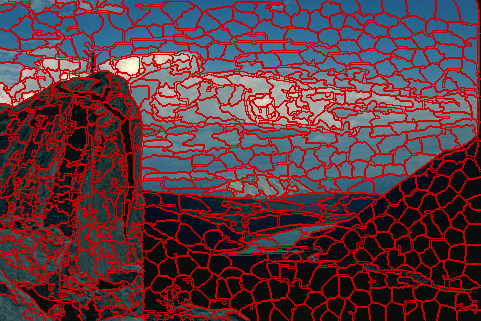
\includegraphics[scale=0.125]{images/bsd-1-reseedssm}
			}
			\subfigure{
				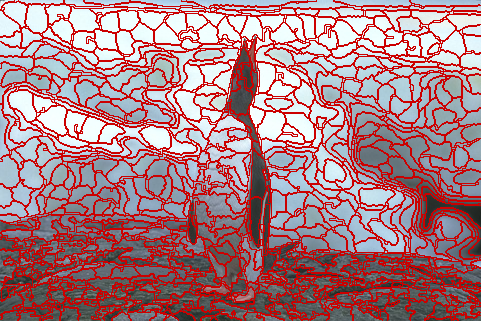
\includegraphics[scale=0.125]{images/bsd-2-reseedssm}
			}
			\subfigure{
				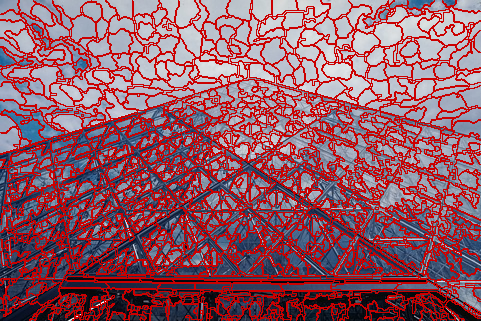
\includegraphics[scale=0.125]{images/bsd-3-reseedssm}
			}
			\subfigure{
				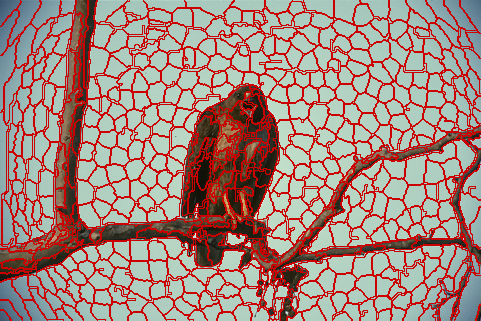
\includegraphics[scale=0.125]{images/bsd-4-reseedssm}
			}
			\subfigure{
				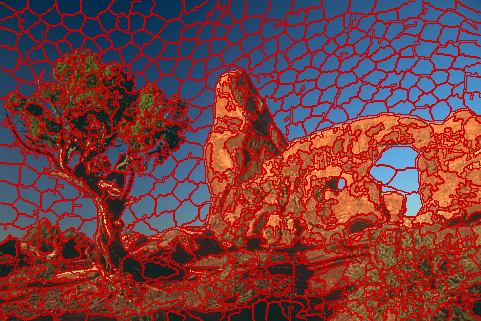
\includegraphics[scale=0.125]{images/bsd-5-reseedssm}
			}
		\end{figure}
		\vskip 0.25cm
		
		\begin{center}
			{\LARGE Questions?}
		\end{center}
	\end{frame}

	\section*{Appendix}
	\begin{frame}{Appendix -- SEEDS}
		\vspace{-0.7cm}
		\begin{algo}{SEEDS}{\label{algo:superpixel-segmentation-seeds}\qinput{image $I$, block size $w \times h$, levels $L$, histogram size $Q$}\qoutput{superpixel segmentation $S$}}{0}
			\qcom{Initialization:}\\
			group $w \times h$ pixels to form blocks at level $l = 1$\\
			\qfor $l = 2$ \qto $L$\\
				group $2 \times 2$ blocks at level $(l - 1)$ to form blocks at level $l$\qrof\\
			\qfor $l = 1$ \qto $L$\\
				\qcom{For  $l = L$, these are the initial superpixels.}\\
				\qforeach block $B_i^{(l)}$ at level $l$\\
					\qcom{$h_{B_i^{(l)}}(q)$ is the fraction of pixels in $B_i^{(l)}$ falling in bin $q$.}\\
					compute color histogram $h_{B_i^{(l)}}$\qrof\qrof
		\end{algo}
	\end{frame}
	
	\begin{frame}{Appendix -- SEEDS}
		\begin{algo}{SEEDS}{\label{algo:superpixel-segmentation-seeds}\qinput{image $I$, block size $w^{(1)} \times h^{(1)}$, levels $L$, histogram size $Q$}\qoutput{superpixel segmentation $S$}}{9}
			\qcom{Block updates:}\\
			\qfor $l = L - 1$ \qto $1$\\
				\qforeach block $B_i^{(l)}$ at level $l$\\
					let $S_j$ be the superpixel $B_i^{(l)}$ belongs to\\
					\qif a neighboring block belongs to a different superpixel $S_k$\\
						\qcom{$\cap(h,h') = \sum_{q=1}^Q \min(h(q), h'(q))$.}\\
						\qthen \qif $\cap(h_{B_i^{(l)}}, h_{S_k}) > \cap(h_{B_i^{(l)}}, h_{S_j - B_i^{(l)}})$\\
							\qthen assign $B_i^{(l)}$ to superpixel $S_k$\qfi\qfi\qrof\qrof
		\end{algo}
	\end{frame}
	
	\begin{frame}{Appendix -- SEEDS}
		\begin{algo}{SEEDS}{\label{algo:superpixel-segmentation-seeds}\qinput{image $I$, block size $w^{(1)} \times h^{(1)}$, levels $L$, histogram size $Q$}\qoutput{superpixel segmentation $S$}}{17}
			\qcom{Pixel updates:}\\
			\qfor $n = 1$ \qto $N$\\
				let $S_j$ be the superpixel $x_n$ belongs to\\
				\qif a neighboring pixel belongs to a different superpixel $S_k$\\
					\qcom{$h(x_n)$ denotes the bin of pixel $x_n$.}\\
					\qthen\qif $h_{S_k}(h(x_n)) > h_{S_j}(h(x_n))$\\
						\qthen assign $x_n$ to superpixel $S_k$\qfi\qfi\qrof\\
			\qreturn $S$
		\end{algo}
	\end{frame}
	
	\begin{frame}{Appendix -- SEEDS}
		\begin{algo}{SEEDS}{\label{algo:superpixel-segmentation-seeds}\qinput{image $I$, block size $w^{(1)} \times h^{(1)}$, levels $L$, histogram size $Q$}\qoutput{superpixel segmentation $S$}}{18}
			\qcom{Mean pixel updates:}\\
			\qfor $n = 1$ \qto $N$\\
				let $S_j$ be the superpixel $x_n$ belongs to\\
				\qif a neighboring pixel belongs to a different superpixel $S_k$\\
					\qcom{$d(x_n, S_j) = \|I(x_n) - I(S_j)\|_2 + \beta \|x_n - \mu(S_j)\|_2$.}\\
					\qthen\qif $d(x_n, S_k) < d(x_n, S_j)$\\
						\qthen assign $x_n$ to superpixel $S_k$\qfi\qfi\qrof\\
			\qreturn $S$
		\end{algo}
	\end{frame}
	
	\begin{frame}{Appendix -- Comparison -- BSDS500}
		\vspace{-0.5cm}
		\begin{figure}
			\centering
			\subfigure{
				\begin{tikzpicture}
					\begin{axis}[
						height=7cm,
						width=4cm,
						xlabel=Superpixels,
						ylabel=$Rec$,
						ymin=0.9,
						ymax=1,
						ytick={0.91,0.92,0.94,0.96,0.98,1},
						xmin=100,
						xmax=1200,
						cycle list name=comparison bsd full]
					
						% FH
						\addplot+[thick] table [row sep=newline,trim cells=true,x=K,y=Rec] {data/fh-bsd-test.csv};
						\label{plot:evaluation-appendix-comparison-fh-rec-bsd}
						
						% TP
						\addplot+[thick] table [row sep=newline,trim cells=true,x=K,y=Rec] {data/tp-bsd-test.csv};
						\label{plot:evaluation-appendix-comparison-tp-rec-bsd}
						
						% SLIC
						\addplot+[thick] table [row sep=newline,trim cells=true,x=K,y=Rec] {data/orislic-bsd-test.csv};
						\label{plot:evaluation-appendix-comparison-orislic-rec-bsd}
					
						% ERS
						\addplot+[thick] table [row sep=newline,trim cells=true,x=K,y=Rec] {data/ers-bsd-test.csv};
						\label{plot:evaluation-appendix-comparison-ers-rec-bsd}
						
						% oriSEEDSmp
						\addplot+[thick] table [row sep=newline,trim cells=true,x=K,y=Rec] {data/oriseedsmp-bsd-test.csv};	
						\label{plot:evaluation-appendix-comparison-oriseedsmp-rec-bsd}
					
						% reSEEDSmp*
						\addplot+[thick] table [row sep=newline,trim cells=true,x=K,y=Rec] {data/reseedssm-bsd-test.csv};
						\label{plot:evaluation-appendix-comparison-reseedssm-rec-bsd}
					
					\end{axis}
				\end{tikzpicture}
			}
			\subfigure{
				\begin{tikzpicture}
					\begin{axis}[
						height=7cm,
						width=4cm,
						xlabel=Superpixels,
						ylabel=$UE$,
						ymin=0.03,
						ymax=0.1,
						ytick={0.03,0.04,0.06,0.08,0.1},
						xmin=100,
						xmax=1200,
						cycle list name=comparison bsd full]
					
						% FH
						\addplot+[thick] table [row sep=newline,trim cells=true,x=K,y=UE] {data/fh-bsd-test.csv};
						\label{plot:evaluation-appendix-comparison-fh-ue-bsd}
					
						% TP
						\addplot+[thick] table [row sep=newline,trim cells=true,x=K,y=UE] {data/tp-bsd-test.csv};
						\label{plot:evaluation-appendix-comparison-tp-ue-bsd}
					
						% SLIC
						\addplot+[thick] table [row sep=newline,trim cells=true,x=K,y=UE] {data/orislic-bsd-test.csv};
						\label{plot:evaluation-appendix-comparison-orislic-ue-bsd}
					
						% ERS
						\addplot+[thick] table [row sep=newline,trim cells=true,x=K,y=UE] {data/ers-bsd-test.csv};
						\label{plot:evaluation-appendix-comparison-ers-ue-bsd}
					
						% oriSEEDSmp
						\addplot+[thick] table [row sep=newline,trim cells=true,x=K,y=UE] {data/oriseedsmp-bsd-test.csv};	
						\label{plot:evaluation-appendix-comparison-oriseedsmp-ue-bsd}
					
						% reSEEDSmp*
						\addplot+[thick] table [row sep=newline,trim cells=true,x=K,y=UE] {data/reseedssm-bsd-test.csv};
						\label{plot:evaluation-appendix-comparison-reseedssm-ue-bsd}
					
					\end{axis}
					\matrix[%
							matrix of nodes,%
							anchor=north west,%
							inner sep=0.25em,%
							nodes={font=\small},%
							column 1/.append style={anchor=base west},%
						] at ($(current axis.north east) + (0.25,0)$) {
							NYUV2:\\
							\ref{plot:evaluation-appendix-comparison-fh-ue-bsd} \textbf{FH}\\
							\ref{plot:evaluation-appendix-comparison-tp-ue-bsd} \textbf{TP}\\
							\ref{plot:evaluation-appendix-comparison-orislic-ue-bsd} \textbf{SLIC}\\
							\ref{plot:evaluation-appendix-comparison-ers-ue-bsd} \textbf{ERS}\\
							\ref{plot:evaluation-appendix-comparison-oriseedsmp-ue-bsd} \textbf{oriSEEDS}\\
							\ref{plot:evaluation-appendix-comparison-reseedssm-ue-bsd} \textbf{reSEEDS*}\\
						};
				\end{tikzpicture}
			}
		\end{figure}
	\end{frame}
	
	\begin{frame}{Appendix -- Comparison -- NYUV2}
		\vspace{-0.5cm}
		\begin{figure}
			\centering
			\subfigure{
				\begin{tikzpicture}
					\begin{axis}[
						height=7cm,
						width=4cm,
						xlabel=Superpixels,
						ylabel=$Rec$,
						ymin=0.91,
						ymax=1,
						ytick={0.91,0.92,0.94,0.96,0.98,1},
						xmin=300,
						xmax=1700,
						cycle list name=comparison nyu full]
					
						% FH
						\addplot+[thick] table [row sep=newline,trim cells=true,x=K,y=Rec] {data/fh-nyu-test.csv};
						\label{plot:evaluation-appendix-comparison-fh-rec-nyu}
						
						% TP
						\addplot+[thick] table [row sep=newline,trim cells=true,x=K,y=Rec] {data/tp-nyu-test.csv};
						\label{plot:evaluation-appendix-comparison-tp-rec-nyu}
						
						% SLIC
						\addplot+[thick] table [row sep=newline,trim cells=true,x=K,y=Rec] {data/orislic-nyu-test.csv};
						\label{plot:evaluation-appendix-comparison-orislic-rec-nyu}
					
						% ERS
						\addplot+[thick] table [row sep=newline,trim cells=true,x=K,y=Rec] {data/ers-nyu-test.csv};
						\label{plot:evaluation-appendix-comparison-ers-rec-nyu}
						
						% oriSEEDSmp
						\addplot+[thick] table [row sep=newline,trim cells=true,x=K,y=Rec] {data/oriseedsmp-nyu-test.csv};	
						\label{plot:evaluation-appendix-comparison-oriseedsmp-rec-nyu}
					
						% reSEEDSmp*
						\addplot+[thick] table [row sep=newline,trim cells=true,x=K,y=Rec] {data/reseedssm-nyu-test.csv};
						\label{plot:evaluation-appendix-comparison-reseedssm-rec-nyu}
					
						% SEEDS3D
						\addplot+[thick] table [row sep=newline,trim cells=true,x=K,y=Rec] {data/seeds3d-nyu-test.csv};
						\label{plot:evaluation-appendix-comparison-seeds3d-rec-nyu}
					
						% DASP
						\addplot+[thick] table [row sep=newline,trim cells=true,x=K,y=Rec] {data/dasp-nyu-test.csv};
						\label{plot:evaluation-appendix-comparison-dasp-rec-nyu}
						
						% VCCS
						\addplot+[thick] table [row sep=newline,trim cells=true,x=K,y=Rec] {data/vccs-depth-test.csv};
						\label{plot:evaluation-appendix-comparison-vccs-rec-nyu}
					
					\end{axis}
				\end{tikzpicture}
			}
			\subfigure{
				\begin{tikzpicture}
					\begin{axis}[
						height=7cm,
						width=4cm,
						xlabel=Superpixels,
						ylabel=$UE$,
						ymin=0.07,
						ymax=0.19,
						ytick={0.07,0.08,0.1,0.12,0.14,0.16,0.18,0.19},
						xmin=300,
						xmax=1700,
						cycle list name=comparison nyu full]
					
						% FH
						\addplot+[thick] table [row sep=newline,trim cells=true,x=K,y=UE] {data/fh-nyu-test.csv};
						\label{plot:evaluation-appendix-comparison-fh-ue-nyu}
					
						% TP
						\addplot+[thick] table [row sep=newline,trim cells=true,x=K,y=UE] {data/tp-nyu-test.csv};
						\label{plot:evaluation-appendix-comparison-tp-ue-nyu}
					
						% SLIC
						\addplot+[thick] table [row sep=newline,trim cells=true,x=K,y=UE] {data/orislic-nyu-test.csv};
						\label{plot:evaluation-appendix-comparison-orislic-ue-nyu}
					
						% ERS
						\addplot+[thick] table [row sep=newline,trim cells=true,x=K,y=UE] {data/ers-nyu-test.csv};
						\label{plot:evaluation-appendix-comparison-ers-ue-nyu}
					
						% oriSEEDSmp
						\addplot+[thick] table [row sep=newline,trim cells=true,x=K,y=UE] {data/oriseedsmp-nyu-test.csv};	
						\label{plot:evaluation-appendix-comparison-oriseedsmp-ue-nyu}
					
						% reSEEDSmp*
						\addplot+[thick] table [row sep=newline,trim cells=true,x=K,y=UE] {data/reseedssm-nyu-test.csv};
						\label{plot:evaluation-appendix-comparison-reseedssm-ue-nyu}
					
						% SEEDS3D
						\addplot+[thick] table [row sep=newline,trim cells=true,x=K,y=UE] {data/seeds3d-nyu-test.csv};
						\label{plot:evaluation-appendix-comparison-seeds3d-ue-nyu}
					
						% VCCS
						\addplot+[thick] table [row sep=newline,trim cells=true,x=K,y=UE] {data/dasp-nyu-test.csv};
						\label{plot:evaluation-appendix-comparison-dasp-ue-nyu}
					
						% VCCS
						\addplot+[thick] table [row sep=newline,trim cells=true,x=K,y=UE] {data/vccs-depth-test.csv};
						\label{plot:evaluation-appendix-comparison-vccs-ue-nyu}
					
					\end{axis}
					\matrix[%
							matrix of nodes,%
							anchor=north west,%
							inner sep=0.25em,%
							nodes={font=\small},%
							column 1/.append style={anchor=base west},%
						] at ($(current axis.north east) + (0.25,0)$) {
							NYUV2:\\
							\ref{plot:evaluation-appendix-comparison-fh-ue-nyu} \textbf{FH}\\
							\ref{plot:evaluation-appendix-comparison-tp-ue-nyu} \textbf{TP}\\
							\ref{plot:evaluation-appendix-comparison-orislic-ue-nyu} \textbf{SLIC}\\
							\ref{plot:evaluation-appendix-comparison-ers-ue-nyu} \textbf{ERS}\\
							\ref{plot:evaluation-appendix-comparison-oriseedsmp-ue-nyu} \textbf{oriSEEDS}\\
							\ref{plot:evaluation-appendix-comparison-reseedssm-ue-nyu} \textbf{reSEEDS*}\\
							\ref{plot:evaluation-appendix-comparison-seeds3d-ue-nyu} \textbf{SEEDS3D}\\
							\ref{plot:evaluation-appendix-comparison-dasp-ue-nyu} \textbf{DASP}\\
							\ref{plot:evaluation-appendix-comparison-vccs-ue-nyu} \textbf{VCCS}\\
						};
				\end{tikzpicture}
			}
		\end{figure}
	\end{frame}
	
	\begin{frame}{Appendix -- Runtime}
		It can be shown that \textbf{SEEDS} runs linear in the number of pixels $N$:
		\begin{align}
			\mathcal{O}(QTN)
		\end{align}
		with
		\begin{itemize}[label=--]
			\item $Q$ the number of histogram bins,
			\item $T$ the number of iterations at each level.
		\end{itemize}
		\vskip 0.5cm
		\pause
		
		However, in practice, the runtime also depends on the number of levels~$L$!
	\end{frame}
	
	\begin{frame}{Appendix -- Runtime}
		\vspace{-0.5cm}
		\begin{figure}
			\centering
			\subfigure{
				\begin{tikzpicture}
					\begin{axis}[
							height=6.5cm,
							width=4cm,
							xlabel=Superpixels,
							ylabel=$t$,
							ymin=0,
							ymax=0.35,
							ytick={0,0.03,0.05,0.1,0.2,0.3,0.35},
							xmin=100,
							xmax=1200,
							cycle list name=low runtime bsd 2]
					
						% SLIC
						\addplot+[thick] table [row sep=newline,trim cells=true,x=K,y=t] {data/orislic-bsd-test.csv};
						\label{plot:evaluation-comparison-orislic-t-bsd}
					
						% oriSEEDSmp
						\addplot+[thick] table [row sep=newline,trim cells=true,x=K,y=t] {data/oriseedsmp-bsd-test.csv};
						\label{plot:evaluation-comparison-oriseedsmp-t-bsd}
					
						% reSEEDSmp*
						\addplot+[thick] table [row sep=newline,trim cells=true,x=K,y=t] {data/reseedssm-bsd-test.csv};
						\label{plot:evaluation-comparison-reseedssm-t-bsd}
					
						% SLIC
						\addplot+[thick] table [row sep=newline,trim cells=true,x=K,y=t] {data/orislic1it-bsd-test.csv};
						\label{plot:evaluation-comparison-orislic1it-t-bsd}
					
						% oriSEEDSmp
						\addplot+[thick] table [row sep=newline,trim cells=true,x=K,y=t] {data/oriseedsmp1it-bsd-test.csv};
						\label{plot:evaluation-comparison-oriseedsmp1it-t-bsd}
					
						% reSEEDSmp*
						\addplot+[thick] table [row sep=newline,trim cells=true,x=K,y=t] {data/reseedssm1it-bsd-test.csv};
						\label{plot:evaluation-comparison-reseedssm1it-t-bsd}
					
					\end{axis}
					\matrix[%
							matrix of nodes,%
							anchor=south west,%
							inner sep=0.25em,%
							nodes={font=\small},%
							column 1/.append style={anchor=base west},%
						] at ($(current axis.north west) + (0,0.1)$) {
							BSDS500\\
					};
				\end{tikzpicture}
			}
			\subfigure{
				\begin{tikzpicture}
					\begin{axis}[
							height=6.5cm,
							width=4cm,
							xlabel=Superpixels,
							ylabel=$t$,
							ymin=0,
							ymax=0.45,
							ytick={0,0.05,0.1,0.2,0.4,0.45},
							xmin=300,
							xmax=1700,
							cycle list name=low runtime nyu 2]
					
						% SLIC
						\addplot+[thick] table [row sep=newline,trim cells=true,x=K,y=t] {data/orislic-nyu-test.csv};
						\label{plot:evaluation-comparison-orislic-t-nyu}
					
						% oriSEEDSmp
						\addplot+[thick] table [row sep=newline,trim cells=true,x=K,y=t] {data/oriseedsmp-nyu-test.csv};
						\label{plot:evaluation-comparison-oriseedsmp-t-nyu}
					
						% reSEEDSmp*
						\addplot+[thick] table [row sep=newline,trim cells=true,x=K,y=t] {data/reseedssm-nyu-test.csv};
						\label{plot:evaluation-comparison-reseedssm-t-nyu}
					
						% SLIC
						\addplot+[thick] table [row sep=newline,trim cells=true,x=K,y=t] {data/orislic1it-nyu-test.csv};
						\label{plot:evaluation-comparison-orislic1it-t-nyu}
					
						% oriSEEDSmp
						\addplot+[thick] table [row sep=newline,trim cells=true,x=K,y=t] {data/oriseedsmp1it-nyu-test.csv};	
						\label{plot:evaluation-comparison-oriseedsmp1it-t-nyu}
					
						% reSEEDSmp*
						\addplot+[thick] table [row sep=newline,trim cells=true,x=K,y=t] {data/reseedssm1it-nyu-test.csv};
						\label{plot:evaluation-comparison-reseedssm1it-t-nyu}
					
					\end{axis}
					\matrix[%
							matrix of nodes,%
							anchor=north west,%
							inner sep=0.25em,%
							nodes={font=\small},%
							column 1/.append style={anchor=base west},%
						] at ($(current axis.north east) + (0.25,0)$) {
							$T = 10$:\\
							\ref{plot:evaluation-comparison-orislic-t-nyu} \textbf{SLIC}\\
							$T = 1$:\\
							\ref{plot:evaluation-comparison-orislic1it-t-nyu} \textbf{SLIC}\\
							$T = 2$, $Q = 7^3$:\\
							\ref{plot:evaluation-comparison-oriseedsmp-t-nyu} \textbf{oriSEEDS}\\
							\ref{plot:evaluation-comparison-reseedssm-t-nyu} \textbf{reSEEDS*}\\
							$T = 1$, $Q = 3^3$:\\
							\ref{plot:evaluation-comparison-oriseedsmp1it-t-nyu} \textbf{oriSEEDS}\\
							\ref{plot:evaluation-comparison-reseedssm1it-t-nyu} \textbf{reSEEDS*}\\
					};
					\matrix[%
							matrix of nodes,%
							anchor=south west,%
							inner sep=0.25em,%
							nodes={font=\small},%
							column 1/.append style={anchor=base west},%
						] at ($(current axis.north west) + (0,0.1)$) {
							NYUV2\\
					};
				\end{tikzpicture}
			}
		\end{figure}
	\end{frame}
	
	\begin{frame}{Appendix -- Boundary Recall}
		Let $G$ be a ground truth segmentation and $S$ be a superpixel segmentation.
		\vskip 0.25cm
		
		Some definitions \cite{NeubertProtzel:2012}:
		\vskip 0.25cm
		
		\begin{itemize}[label=--]
			\item \textbf{True Positives $TP(G,S)$:} The number of boundary pixels in $G$ for which there is a boundary pixel in $S$ in range $r$.
			\item \textbf{False Negatives $FN(G,S)$:} The number of boundary pixels in $G$ for which there is no boundary pixel in $S$ in range $r$.
		\end{itemize}
		\vskip 0.25cm
		
		Boundary Recall is defined as
		\begin{align}
				Rec(G,S) = \frac{TP(G,S)}{TP(G,S) + FN(G,S)}.
		\end{align}
	\end{frame}
		
	\begin{frame}{Appendix -- Undersegmentation Error}
		Let $G$ be a ground truth segmentation, $S$ be a superpixel segmentation and $N$ be the total number of pixels.
		\vskip 0.25cm
		
		Undersegmentation Error is defined as
		\begin{align}
			UE(G, S) = \frac{1}{N} \left[\sum _{G_i \in G} \sum _{S_j \cap G_i \neq \emptyset} \min (|S_j \cap G_i|, |S_j - G_i|) \right].
		\end{align}
	\end{frame}

%	\begin{frame}{References}
%		\vfill
%		\begin{center}
%			{\Large References}
%		\end{center}
%		\vfill
%	\end{frame}

	\nocite{*}
	\bibliographystyle{alpha}
	\bibliography{slides}
\end{document}